\documentclass[twoside]{book}

% Packages required by doxygen
\usepackage{fixltx2e}
\usepackage{calc}
\usepackage{doxygen}
\usepackage[export]{adjustbox} % also loads graphicx
\usepackage{graphicx}
\usepackage[utf8]{inputenc}
\usepackage{makeidx}
\usepackage{multicol}
\usepackage{multirow}
\PassOptionsToPackage{warn}{textcomp}
\usepackage{textcomp}
\usepackage[nointegrals]{wasysym}
\usepackage[table]{xcolor}

% Font selection
\usepackage[T1]{fontenc}
\usepackage[scaled=.90]{helvet}
\usepackage{courier}
\usepackage{amssymb}
\usepackage{sectsty}
\renewcommand{\familydefault}{\sfdefault}
\allsectionsfont{%
  \fontseries{bc}\selectfont%
  \color{darkgray}%
}
\renewcommand{\DoxyLabelFont}{%
  \fontseries{bc}\selectfont%
  \color{darkgray}%
}
\newcommand{\+}{\discretionary{\mbox{\scriptsize$\hookleftarrow$}}{}{}}

% Page & text layout
\usepackage{geometry}
\geometry{%
  a4paper,%
  top=2.5cm,%
  bottom=2.5cm,%
  left=2.5cm,%
  right=2.5cm%
}
\tolerance=750
\hfuzz=15pt
\hbadness=750
\setlength{\emergencystretch}{15pt}
\setlength{\parindent}{0cm}
\setlength{\parskip}{3ex plus 2ex minus 2ex}
\makeatletter
\renewcommand{\paragraph}{%
  \@startsection{paragraph}{4}{0ex}{-1.0ex}{1.0ex}{%
    \normalfont\normalsize\bfseries\SS@parafont%
  }%
}
\renewcommand{\subparagraph}{%
  \@startsection{subparagraph}{5}{0ex}{-1.0ex}{1.0ex}{%
    \normalfont\normalsize\bfseries\SS@subparafont%
  }%
}
\makeatother

% Headers & footers
\usepackage{fancyhdr}
\pagestyle{fancyplain}
\fancyhead[LE]{\fancyplain{}{\bfseries\thepage}}
\fancyhead[CE]{\fancyplain{}{}}
\fancyhead[RE]{\fancyplain{}{\bfseries\leftmark}}
\fancyhead[LO]{\fancyplain{}{\bfseries\rightmark}}
\fancyhead[CO]{\fancyplain{}{}}
\fancyhead[RO]{\fancyplain{}{\bfseries\thepage}}
\fancyfoot[LE]{\fancyplain{}{}}
\fancyfoot[CE]{\fancyplain{}{}}
\fancyfoot[RE]{\fancyplain{}{\bfseries\scriptsize Generated by Doxygen }}
\fancyfoot[LO]{\fancyplain{}{\bfseries\scriptsize Generated by Doxygen }}
\fancyfoot[CO]{\fancyplain{}{}}
\fancyfoot[RO]{\fancyplain{}{}}
\renewcommand{\footrulewidth}{0.4pt}
\renewcommand{\chaptermark}[1]{%
  \markboth{#1}{}%
}
\renewcommand{\sectionmark}[1]{%
  \markright{\thesection\ #1}%
}

% Indices & bibliography
\usepackage{natbib}
\usepackage[titles]{tocloft}
\setcounter{tocdepth}{3}
\setcounter{secnumdepth}{5}
\makeindex

% Hyperlinks (required, but should be loaded last)
\usepackage{ifpdf}
\ifpdf
  \usepackage[pdftex,pagebackref=true]{hyperref}
\else
  \usepackage[ps2pdf,pagebackref=true]{hyperref}
\fi
\hypersetup{%
  colorlinks=true,%
  linkcolor=blue,%
  citecolor=blue,%
  unicode%
}

% Custom commands
\newcommand{\clearemptydoublepage}{%
  \newpage{\pagestyle{empty}\cleardoublepage}%
}

\usepackage{caption}
\captionsetup{labelsep=space,justification=centering,font={bf},singlelinecheck=off,skip=4pt,position=top}

%===== C O N T E N T S =====

\begin{document}

% Titlepage & ToC
\hypersetup{pageanchor=false,
             bookmarksnumbered=true,
             pdfencoding=unicode
            }
\pagenumbering{alph}
\begin{titlepage}
\vspace*{7cm}
\begin{center}%
{\Large Operação “\+Leva Jeito” }\\
\vspace*{1cm}
{\large Generated by Doxygen 1.8.13}\\
\end{center}
\end{titlepage}
\clearemptydoublepage
\pagenumbering{roman}
\tableofcontents
\clearemptydoublepage
\pagenumbering{arabic}
\hypersetup{pageanchor=true}

%--- Begin generated contents ---
\chapter{Atividade Prática – Operação “\+Leva Jeito”}
\label{md__home_allandemiranda__documentos__hash-_leva-_jeito__r_e_a_d_m_e}
\Hypertarget{md__home_allandemiranda__documentos__hash-_leva-_jeito__r_e_a_d_m_e}
Desenvolvido por \href{https://github.com/allandemiranda}{\tt Allan de Miranda}

25 de setembro de 2019 -\/ Segurança de Redes -\/ I\+MD

\subsection*{Introdução}

Por conta de seus conhecimentos em segurança computacional, você foi convocado a colaborar com as investigações da operação “\+Leva Jeito” na qualidade de concultor técnico.

Sua contribuição inicial será o desenvolvimento de um software que permita garantir a integridade de documentos extraídos de computadores, preservando assim a cadeia de custódia destes elementos de prova.

O problema relatado é que documentos extraídos ou coletados em computadores de suspeitos podem potencialmente serem alterados entre a sua coleta e o seu processamento investigativo.

Assim, a equipe da “\+Leva Jeito” requisitou a você o desenvolvimento de um software que permita verificar a integridade dos dados a qualquer momento.

\subsection*{Implementação}

Implemente o programa guarda que, usando de calculo de puro Hash ou H\+M\+AC, permita garantir a autenticação de um conjunto de arquivos para uma determinada pasta (recursivamente). O programa deverá ser executado em linha de comando, seguindo a sintaxe\+:

./guarda $<$metodo$>$ $<$opcao$>$ $<$pasta$>$ $<$saida$>$

― $<$metodo$>$ \+: indica o método a ser utilizado ( --hash ou --hmac senha) ― $<$opcao$>$\+: indica a ação a ser desempenhada pelo programa • -\/i \+: inicia a guarda da pasta indicada em $<$pasta$>$, ou seja, faz a leitura de todos os arquivos da pasta (recursivamente) registrando os dados e Hash/\+H\+M\+AC de cada um e armazenando numa estrutura própria (Ex\+: tabela hash em uma subpasta oculta ./guarda – ou pode ser usada uma árvore B) • -\/t \+: faz o rastreio (tracking) da pasta indicada em $<$pasta$>$, inserindo informações sobre novos arquivos e indicando alterações detectadas/exclusões • -\/x \+: desativa a guarda e remove a estrutura alocada ― $<$pasta$>$ \+: indica a pasta a ser “guardada” ― $<$saida$>$ \+: indica o arquivo de saída para o relatório (-\/o saída). Caso não seja passado este parâmetro, a saída deve ser feita em tela.

\subsection*{Requisitos}

Para a instalação do programa é necessário que seu computador tenha os seguintes pacotes\+:

{\ttfamily g++ openssl libssl-\/dev libboost-\/all-\/dev}

Para instalar estes pacotes abra o terminal e digite\+:

{\ttfamily sudo apt-\/get install g++ openssl libssl-\/dev libboost-\/all-\/dev}

\subsection*{Instalação}

Para instalar e executar o programa siga as instruções\+:


\begin{DoxyEnumerate}
\item Abra o terminal do seu sistema operacional e digite {\ttfamily cd}
\item {\ttfamily git clone \href{https://github.com/allandemiranda/Hash-Leva-Jeito.git}{\tt https\+://github.\+com/allandemiranda/\+Hash-\/\+Leva-\/\+Jeito.\+git}}
\item {\ttfamily cd Hash-\/\+Leva-\/\+Jeito/}
\item {\ttfamily make}
\end{DoxyEnumerate}

\subsection*{Como utilizar programa \hyperlink{class_guarda}{Guarda}}


\begin{DoxyEnumerate}
\item Abra o terminal do seu sistema operacional e digite {\ttfamily cd}
\item {\ttfamily cd criptografia-\/simetrica/}
\item {\ttfamily ./bin/guarda $<$metodo$>$ $<$opcao$>$ $<$pasta$>$ $<$saída$>$}
\item A utilização destes argumentos de entrada estão descritos no item de implementação. 
\end{DoxyEnumerate}
\chapter{Class Index}
\section{Class List}
Here are the classes, structs, unions and interfaces with brief descriptions\+:\begin{DoxyCompactList}
\item\contentsline{section}{\hyperlink{class_check_hash_table}{Check\+Hash\+Table} }{\pageref{class_check_hash_table}}{}
\item\contentsline{section}{\hyperlink{class_create_hash_table}{Create\+Hash\+Table} }{\pageref{class_create_hash_table}}{}
\item\contentsline{section}{\hyperlink{class_guarda}{Guarda} }{\pageref{class_guarda}}{}
\item\contentsline{section}{\hyperlink{class_hash_file}{Hash\+File} }{\pageref{class_hash_file}}{}
\item\contentsline{section}{\hyperlink{class_log}{Log} }{\pageref{class_log}}{}
\item\contentsline{section}{\hyperlink{class_open_log_file}{Open\+Log\+File} }{\pageref{class_open_log_file}}{}
\item\contentsline{section}{\hyperlink{class_reading_folder_files}{Reading\+Folder\+Files} }{\pageref{class_reading_folder_files}}{}
\item\contentsline{section}{\hyperlink{class_report_output}{Report\+Output} }{\pageref{class_report_output}}{}
\end{DoxyCompactList}

\chapter{File Index}
\section{File List}
Here is a list of all files with brief descriptions\+:\begin{DoxyCompactList}
\item\contentsline{section}{/home/allandemiranda/\+Documentos/\+Hash-\/\+Leva-\/\+Jeito/include/\hyperlink{_check_hash_table_8hpp}{Check\+Hash\+Table.\+hpp} \\*Classe para comparar os arquivos com o da tabela de configuraçao }{\pageref{_check_hash_table_8hpp}}{}
\item\contentsline{section}{/home/allandemiranda/\+Documentos/\+Hash-\/\+Leva-\/\+Jeito/include/\hyperlink{_create_hash_table_8hpp}{Create\+Hash\+Table.\+hpp} \\*Classe para a criação do arquivo de configuração }{\pageref{_create_hash_table_8hpp}}{}
\item\contentsline{section}{/home/allandemiranda/\+Documentos/\+Hash-\/\+Leva-\/\+Jeito/include/\hyperlink{_guarda_8hpp}{Guarda.\+hpp} \\*Classe de controle }{\pageref{_guarda_8hpp}}{}
\item\contentsline{section}{/home/allandemiranda/\+Documentos/\+Hash-\/\+Leva-\/\+Jeito/include/\hyperlink{_hash_file_8hpp}{Hash\+File.\+hpp} \\*Classe que cria a hash para o arquivo solicitado }{\pageref{_hash_file_8hpp}}{}
\item\contentsline{section}{/home/allandemiranda/\+Documentos/\+Hash-\/\+Leva-\/\+Jeito/include/\hyperlink{_log_8hpp}{Log.\+hpp} \\*Classe para gerenciar o modelo de logs }{\pageref{_log_8hpp}}{}
\item\contentsline{section}{/home/allandemiranda/\+Documentos/\+Hash-\/\+Leva-\/\+Jeito/include/\hyperlink{_open_log_file_8hpp}{Open\+Log\+File.\+hpp} \\*Classe para abrir arquivos de log de acordo com o padrão solicitado }{\pageref{_open_log_file_8hpp}}{}
\item\contentsline{section}{/home/allandemiranda/\+Documentos/\+Hash-\/\+Leva-\/\+Jeito/include/\hyperlink{_reading_folder_files_8hpp}{Reading\+Folder\+Files.\+hpp} \\*Classe para gerenciar a leitura de todos os arquivos de todas as pastas }{\pageref{_reading_folder_files_8hpp}}{}
\item\contentsline{section}{/home/allandemiranda/\+Documentos/\+Hash-\/\+Leva-\/\+Jeito/include/\hyperlink{_report_output_8hpp}{Report\+Output.\+hpp} \\*Classe para gerenciar saída de arquivo de log }{\pageref{_report_output_8hpp}}{}
\item\contentsline{section}{/home/allandemiranda/\+Documentos/\+Hash-\/\+Leva-\/\+Jeito/src/\hyperlink{_check_hash_table_8cpp}{Check\+Hash\+Table.\+cpp} \\*Metodos da classe \hyperlink{class_check_hash_table}{Check\+Hash\+Table} }{\pageref{_check_hash_table_8cpp}}{}
\item\contentsline{section}{/home/allandemiranda/\+Documentos/\+Hash-\/\+Leva-\/\+Jeito/src/\hyperlink{_create_hash_table_8cpp}{Create\+Hash\+Table.\+cpp} \\*Métodos para classe \hyperlink{class_create_hash_table}{Create\+Hash\+Table} }{\pageref{_create_hash_table_8cpp}}{}
\item\contentsline{section}{/home/allandemiranda/\+Documentos/\+Hash-\/\+Leva-\/\+Jeito/src/\hyperlink{_guarda_8cpp}{Guarda.\+cpp} \\*Métodos para classe \hyperlink{class_guarda}{Guarda} }{\pageref{_guarda_8cpp}}{}
\item\contentsline{section}{/home/allandemiranda/\+Documentos/\+Hash-\/\+Leva-\/\+Jeito/src/\hyperlink{_hash_file_8cpp}{Hash\+File.\+cpp} \\*Métodos para classe \hyperlink{class_hash_file}{Hash\+File} }{\pageref{_hash_file_8cpp}}{}
\item\contentsline{section}{/home/allandemiranda/\+Documentos/\+Hash-\/\+Leva-\/\+Jeito/src/\hyperlink{_log_8cpp}{Log.\+cpp} \\*Métodos da classe \hyperlink{class_log}{Log} }{\pageref{_log_8cpp}}{}
\item\contentsline{section}{/home/allandemiranda/\+Documentos/\+Hash-\/\+Leva-\/\+Jeito/src/\hyperlink{main_8cpp}{main.\+cpp} \\*Main }{\pageref{main_8cpp}}{}
\item\contentsline{section}{/home/allandemiranda/\+Documentos/\+Hash-\/\+Leva-\/\+Jeito/src/\hyperlink{_open_log_file_8cpp}{Open\+Log\+File.\+cpp} \\*Métodos para a classe \hyperlink{class_open_log_file}{Open\+Log\+File} }{\pageref{_open_log_file_8cpp}}{}
\item\contentsline{section}{/home/allandemiranda/\+Documentos/\+Hash-\/\+Leva-\/\+Jeito/src/\hyperlink{_reading_folder_files_8cpp}{Reading\+Folder\+Files.\+cpp} \\*Métodos da classe \hyperlink{class_reading_folder_files}{Reading\+Folder\+Files} }{\pageref{_reading_folder_files_8cpp}}{}
\item\contentsline{section}{/home/allandemiranda/\+Documentos/\+Hash-\/\+Leva-\/\+Jeito/src/\hyperlink{_report_output_8cpp}{Report\+Output.\+cpp} \\*Métodos para a classe \hyperlink{class_report_output}{Report\+Output} }{\pageref{_report_output_8cpp}}{}
\end{DoxyCompactList}

\chapter{Class Documentation}
\hypertarget{class_check_hash_table}{}\section{Check\+Hash\+Table Class Reference}
\label{class_check_hash_table}\index{Check\+Hash\+Table@{Check\+Hash\+Table}}


{\ttfamily \#include $<$Check\+Hash\+Table.\+hpp$>$}

\subsection*{Public Member Functions}
\begin{DoxyCompactItemize}
\item 
void \hyperlink{class_check_hash_table_a976b114162765decaa1c7fe0b8e16cf8}{show\+Status\+Log} (void)
\begin{DoxyCompactList}\small\item\em Imprimir na tela o vetor status de logs. \end{DoxyCompactList}\item 
std\+::vector$<$ \hyperlink{class_log}{Log} $>$ \hyperlink{class_check_hash_table_ac57b97e1bf321ea232370d1ae0da3a55}{get\+Status\+Log\+Vector} (void)
\begin{DoxyCompactList}\small\item\em Get the Status \hyperlink{class_log}{Log} Vector object. \end{DoxyCompactList}\item 
\hyperlink{class_check_hash_table_a4e5be4b9a124cbf72c8f06d63e6ffca5}{Check\+Hash\+Table} (std\+::vector$<$ std\+::string $>$, std\+::vector$<$ \hyperlink{class_log}{Log} $>$)
\begin{DoxyCompactList}\small\item\em Construct a new Check Hash Table\+:\+: Check Hash Table object. \end{DoxyCompactList}\item 
\hyperlink{class_check_hash_table_a64c43b1e671248aa466b3310471d3d96}{Check\+Hash\+Table} (std\+::vector$<$ std\+::string $>$, std\+::vector$<$ \hyperlink{class_log}{Log} $>$, std\+::string)
\begin{DoxyCompactList}\small\item\em Construct a new Check Hash Table\+:\+: Check Hash Table object. \end{DoxyCompactList}\item 
\hyperlink{class_check_hash_table_ae7cb5a5c4a6ef08a073010f104c3f9df}{$\sim$\+Check\+Hash\+Table} (void)
\end{DoxyCompactItemize}


\subsection{Detailed Description}


Definition at line 19 of file Check\+Hash\+Table.\+hpp.



\subsection{Constructor \& Destructor Documentation}
\mbox{\Hypertarget{class_check_hash_table_a4e5be4b9a124cbf72c8f06d63e6ffca5}\label{class_check_hash_table_a4e5be4b9a124cbf72c8f06d63e6ffca5}} 
\index{Check\+Hash\+Table@{Check\+Hash\+Table}!Check\+Hash\+Table@{Check\+Hash\+Table}}
\index{Check\+Hash\+Table@{Check\+Hash\+Table}!Check\+Hash\+Table@{Check\+Hash\+Table}}
\subsubsection{\texorpdfstring{Check\+Hash\+Table()}{CheckHashTable()}\hspace{0.1cm}{\footnotesize\ttfamily [1/2]}}
{\footnotesize\ttfamily Check\+Hash\+Table\+::\+Check\+Hash\+Table (\begin{DoxyParamCaption}\item[{std\+::vector$<$ std\+::string $>$}]{file\+Table,  }\item[{std\+::vector$<$ \hyperlink{class_log}{Log} $>$}]{log\+Table }\end{DoxyParamCaption})}



Construct a new Check Hash Table\+:\+: Check Hash Table object. 


\begin{DoxyParams}{Parameters}
{\em file\+Table} & Tabela de arquivos da pasta \\
\hline
{\em log\+Table} & Tabela de log existente \\
\hline
\end{DoxyParams}


Definition at line 26 of file Check\+Hash\+Table.\+cpp.

Here is the call graph for this function\+:
\nopagebreak
\begin{figure}[H]
\begin{center}
\leavevmode

\includegraphics[width=350pt]{dc/d2a/class_check_hash_table_a4e5be4b9a124cbf72c8f06d63e6ffca5_cgraph}
\end{center}
\end{figure}
\mbox{\Hypertarget{class_check_hash_table_a64c43b1e671248aa466b3310471d3d96}\label{class_check_hash_table_a64c43b1e671248aa466b3310471d3d96}} 
\index{Check\+Hash\+Table@{Check\+Hash\+Table}!Check\+Hash\+Table@{Check\+Hash\+Table}}
\index{Check\+Hash\+Table@{Check\+Hash\+Table}!Check\+Hash\+Table@{Check\+Hash\+Table}}
\subsubsection{\texorpdfstring{Check\+Hash\+Table()}{CheckHashTable()}\hspace{0.1cm}{\footnotesize\ttfamily [2/2]}}
{\footnotesize\ttfamily Check\+Hash\+Table\+::\+Check\+Hash\+Table (\begin{DoxyParamCaption}\item[{std\+::vector$<$ std\+::string $>$}]{file\+Table,  }\item[{std\+::vector$<$ \hyperlink{class_log}{Log} $>$}]{log\+Table,  }\item[{std\+::string}]{key }\end{DoxyParamCaption})}



Construct a new Check Hash Table\+:\+: Check Hash Table object. 


\begin{DoxyParams}{Parameters}
{\em file\+Table} & Tabela de arquivos da pasta \\
\hline
{\em log\+Table} & Tabela de log existente \\
\hline
{\em key} & Chave \\
\hline
\end{DoxyParams}


Definition at line 61 of file Check\+Hash\+Table.\+cpp.

Here is the call graph for this function\+:
\nopagebreak
\begin{figure}[H]
\begin{center}
\leavevmode

\includegraphics[width=350pt]{dc/d2a/class_check_hash_table_a64c43b1e671248aa466b3310471d3d96_cgraph}
\end{center}
\end{figure}
\mbox{\Hypertarget{class_check_hash_table_ae7cb5a5c4a6ef08a073010f104c3f9df}\label{class_check_hash_table_ae7cb5a5c4a6ef08a073010f104c3f9df}} 
\index{Check\+Hash\+Table@{Check\+Hash\+Table}!````~Check\+Hash\+Table@{$\sim$\+Check\+Hash\+Table}}
\index{````~Check\+Hash\+Table@{$\sim$\+Check\+Hash\+Table}!Check\+Hash\+Table@{Check\+Hash\+Table}}
\subsubsection{\texorpdfstring{$\sim$\+Check\+Hash\+Table()}{~CheckHashTable()}}
{\footnotesize\ttfamily Check\+Hash\+Table\+::$\sim$\+Check\+Hash\+Table (\begin{DoxyParamCaption}\item[{void}]{ }\end{DoxyParamCaption})}



Definition at line 89 of file Check\+Hash\+Table.\+cpp.



\subsection{Member Function Documentation}
\mbox{\Hypertarget{class_check_hash_table_ac57b97e1bf321ea232370d1ae0da3a55}\label{class_check_hash_table_ac57b97e1bf321ea232370d1ae0da3a55}} 
\index{Check\+Hash\+Table@{Check\+Hash\+Table}!get\+Status\+Log\+Vector@{get\+Status\+Log\+Vector}}
\index{get\+Status\+Log\+Vector@{get\+Status\+Log\+Vector}!Check\+Hash\+Table@{Check\+Hash\+Table}}
\subsubsection{\texorpdfstring{get\+Status\+Log\+Vector()}{getStatusLogVector()}}
{\footnotesize\ttfamily std\+::vector$<$ \hyperlink{class_log}{Log} $>$ Check\+Hash\+Table\+::get\+Status\+Log\+Vector (\begin{DoxyParamCaption}\item[{void}]{ }\end{DoxyParamCaption})}



Get the Status \hyperlink{class_log}{Log} Vector object. 

\begin{DoxyReturn}{Returns}
std\+::vector$<$\+Log$>$ Vetor com os logs finais 
\end{DoxyReturn}


Definition at line 107 of file Check\+Hash\+Table.\+cpp.

\mbox{\Hypertarget{class_check_hash_table_a976b114162765decaa1c7fe0b8e16cf8}\label{class_check_hash_table_a976b114162765decaa1c7fe0b8e16cf8}} 
\index{Check\+Hash\+Table@{Check\+Hash\+Table}!show\+Status\+Log@{show\+Status\+Log}}
\index{show\+Status\+Log@{show\+Status\+Log}!Check\+Hash\+Table@{Check\+Hash\+Table}}
\subsubsection{\texorpdfstring{show\+Status\+Log()}{showStatusLog()}}
{\footnotesize\ttfamily void Check\+Hash\+Table\+::show\+Status\+Log (\begin{DoxyParamCaption}\item[{void}]{ }\end{DoxyParamCaption})}



Imprimir na tela o vetor status de logs. 



Definition at line 115 of file Check\+Hash\+Table.\+cpp.

Here is the caller graph for this function\+:
\nopagebreak
\begin{figure}[H]
\begin{center}
\leavevmode
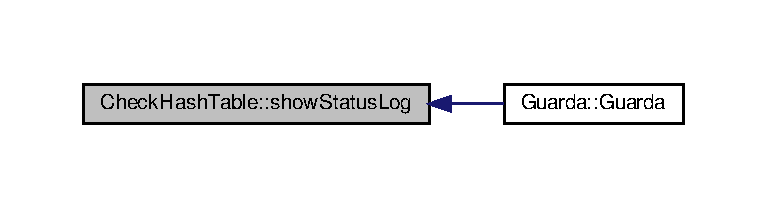
\includegraphics[width=350pt]{dc/d2a/class_check_hash_table_a976b114162765decaa1c7fe0b8e16cf8_icgraph}
\end{center}
\end{figure}


The documentation for this class was generated from the following files\+:\begin{DoxyCompactItemize}
\item 
/home/allandemiranda/\+Documentos/\+Hash-\/\+Leva-\/\+Jeito/include/\hyperlink{_check_hash_table_8hpp}{Check\+Hash\+Table.\+hpp}\item 
/home/allandemiranda/\+Documentos/\+Hash-\/\+Leva-\/\+Jeito/src/\hyperlink{_check_hash_table_8cpp}{Check\+Hash\+Table.\+cpp}\end{DoxyCompactItemize}

\hypertarget{class_create_hash_table}{}\section{Create\+Hash\+Table Class Reference}
\label{class_create_hash_table}\index{Create\+Hash\+Table@{Create\+Hash\+Table}}


{\ttfamily \#include $<$Create\+Hash\+Table.\+hpp$>$}

\subsection*{Public Member Functions}
\begin{DoxyCompactItemize}
\item 
void \hyperlink{class_create_hash_table_ab50343628947f7064f4ab646a834ef03}{show\+Log} (void)
\begin{DoxyCompactList}\small\item\em Mostar o log da tabela criada. \end{DoxyCompactList}\item 
std\+::vector$<$ \hyperlink{class_log}{Log} $>$ \hyperlink{class_create_hash_table_a9e01964c0d11a330bfce92c77fad0ca5}{get\+Hash\+Table} (void)
\begin{DoxyCompactList}\small\item\em Get the Hash Table object. \end{DoxyCompactList}\item 
\hyperlink{class_create_hash_table_a9cc25111eb98da7c68ff4dcff9cdd4ea}{Create\+Hash\+Table} (std\+::vector$<$ std\+::string $>$)
\begin{DoxyCompactList}\small\item\em Create a Hash Table\+:\+: Create Hash Table object. \end{DoxyCompactList}\item 
\hyperlink{class_create_hash_table_a3aac5164fee71508dbd12eaa4c81ab44}{Create\+Hash\+Table} (std\+::vector$<$ std\+::string $>$, std\+::string)
\begin{DoxyCompactList}\small\item\em Create a Hash Table object. \end{DoxyCompactList}\item 
\hyperlink{class_create_hash_table_abf22158361dd73d04edf1739ef6b3482}{$\sim$\+Create\+Hash\+Table} (void)
\begin{DoxyCompactList}\small\item\em Create a Hash Table\+:\+:$\sim$ Create Hash Table object. \end{DoxyCompactList}\end{DoxyCompactItemize}


\subsection{Detailed Description}


Definition at line 19 of file Create\+Hash\+Table.\+hpp.



\subsection{Constructor \& Destructor Documentation}
\mbox{\Hypertarget{class_create_hash_table_a9cc25111eb98da7c68ff4dcff9cdd4ea}\label{class_create_hash_table_a9cc25111eb98da7c68ff4dcff9cdd4ea}} 
\index{Create\+Hash\+Table@{Create\+Hash\+Table}!Create\+Hash\+Table@{Create\+Hash\+Table}}
\index{Create\+Hash\+Table@{Create\+Hash\+Table}!Create\+Hash\+Table@{Create\+Hash\+Table}}
\subsubsection{\texorpdfstring{Create\+Hash\+Table()}{CreateHashTable()}\hspace{0.1cm}{\footnotesize\ttfamily [1/2]}}
{\footnotesize\ttfamily Create\+Hash\+Table\+::\+Create\+Hash\+Table (\begin{DoxyParamCaption}\item[{std\+::vector$<$ std\+::string $>$}]{path }\end{DoxyParamCaption})}



Create a Hash Table\+:\+: Create Hash Table object. 


\begin{DoxyParams}{Parameters}
{\em path} & Vetor de caminho de arquivos \\
\hline
\end{DoxyParams}


Definition at line 25 of file Create\+Hash\+Table.\+cpp.

Here is the call graph for this function\+:
\nopagebreak
\begin{figure}[H]
\begin{center}
\leavevmode

\includegraphics[width=350pt]{d9/d9e/class_create_hash_table_a9cc25111eb98da7c68ff4dcff9cdd4ea_cgraph}
\end{center}
\end{figure}
\mbox{\Hypertarget{class_create_hash_table_a3aac5164fee71508dbd12eaa4c81ab44}\label{class_create_hash_table_a3aac5164fee71508dbd12eaa4c81ab44}} 
\index{Create\+Hash\+Table@{Create\+Hash\+Table}!Create\+Hash\+Table@{Create\+Hash\+Table}}
\index{Create\+Hash\+Table@{Create\+Hash\+Table}!Create\+Hash\+Table@{Create\+Hash\+Table}}
\subsubsection{\texorpdfstring{Create\+Hash\+Table()}{CreateHashTable()}\hspace{0.1cm}{\footnotesize\ttfamily [2/2]}}
{\footnotesize\ttfamily Create\+Hash\+Table\+::\+Create\+Hash\+Table (\begin{DoxyParamCaption}\item[{std\+::vector$<$ std\+::string $>$}]{path,  }\item[{std\+::string}]{key }\end{DoxyParamCaption})}



Create a Hash Table object. 


\begin{DoxyParams}{Parameters}
{\em path} & Vetor de caminho de arquivos \\
\hline
{\em key} & Chave \\
\hline
\end{DoxyParams}


Definition at line 40 of file Create\+Hash\+Table.\+cpp.

Here is the call graph for this function\+:
\nopagebreak
\begin{figure}[H]
\begin{center}
\leavevmode

\includegraphics[width=350pt]{d9/d9e/class_create_hash_table_a3aac5164fee71508dbd12eaa4c81ab44_cgraph}
\end{center}
\end{figure}
\mbox{\Hypertarget{class_create_hash_table_abf22158361dd73d04edf1739ef6b3482}\label{class_create_hash_table_abf22158361dd73d04edf1739ef6b3482}} 
\index{Create\+Hash\+Table@{Create\+Hash\+Table}!````~Create\+Hash\+Table@{$\sim$\+Create\+Hash\+Table}}
\index{````~Create\+Hash\+Table@{$\sim$\+Create\+Hash\+Table}!Create\+Hash\+Table@{Create\+Hash\+Table}}
\subsubsection{\texorpdfstring{$\sim$\+Create\+Hash\+Table()}{~CreateHashTable()}}
{\footnotesize\ttfamily Create\+Hash\+Table\+::$\sim$\+Create\+Hash\+Table (\begin{DoxyParamCaption}\item[{void}]{ }\end{DoxyParamCaption})}



Create a Hash Table\+:\+:$\sim$ Create Hash Table object. 



Definition at line 54 of file Create\+Hash\+Table.\+cpp.



\subsection{Member Function Documentation}
\mbox{\Hypertarget{class_create_hash_table_a9e01964c0d11a330bfce92c77fad0ca5}\label{class_create_hash_table_a9e01964c0d11a330bfce92c77fad0ca5}} 
\index{Create\+Hash\+Table@{Create\+Hash\+Table}!get\+Hash\+Table@{get\+Hash\+Table}}
\index{get\+Hash\+Table@{get\+Hash\+Table}!Create\+Hash\+Table@{Create\+Hash\+Table}}
\subsubsection{\texorpdfstring{get\+Hash\+Table()}{getHashTable()}}
{\footnotesize\ttfamily std\+::vector$<$ \hyperlink{class_log}{Log} $>$ Create\+Hash\+Table\+::get\+Hash\+Table (\begin{DoxyParamCaption}\item[{void}]{ }\end{DoxyParamCaption})}



Get the Hash Table object. 

\begin{DoxyReturn}{Returns}
std\+::vector$<$\+Log$>$ Vetor de logs gerado 
\end{DoxyReturn}


Definition at line 70 of file Create\+Hash\+Table.\+cpp.

\mbox{\Hypertarget{class_create_hash_table_ab50343628947f7064f4ab646a834ef03}\label{class_create_hash_table_ab50343628947f7064f4ab646a834ef03}} 
\index{Create\+Hash\+Table@{Create\+Hash\+Table}!show\+Log@{show\+Log}}
\index{show\+Log@{show\+Log}!Create\+Hash\+Table@{Create\+Hash\+Table}}
\subsubsection{\texorpdfstring{show\+Log()}{showLog()}}
{\footnotesize\ttfamily void Create\+Hash\+Table\+::show\+Log (\begin{DoxyParamCaption}\item[{void}]{ }\end{DoxyParamCaption})}



Mostar o log da tabela criada. 



Definition at line 76 of file Create\+Hash\+Table.\+cpp.

Here is the caller graph for this function\+:
\nopagebreak
\begin{figure}[H]
\begin{center}
\leavevmode
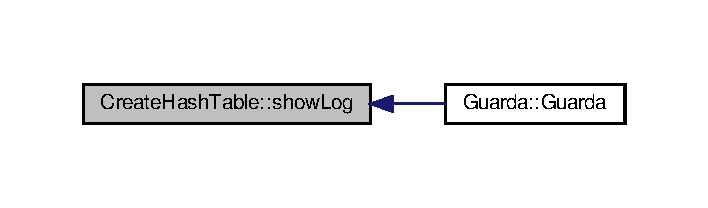
\includegraphics[width=340pt]{d9/d9e/class_create_hash_table_ab50343628947f7064f4ab646a834ef03_icgraph}
\end{center}
\end{figure}


The documentation for this class was generated from the following files\+:\begin{DoxyCompactItemize}
\item 
/home/allandemiranda/\+Documentos/\+Hash-\/\+Leva-\/\+Jeito/include/\hyperlink{_create_hash_table_8hpp}{Create\+Hash\+Table.\+hpp}\item 
/home/allandemiranda/\+Documentos/\+Hash-\/\+Leva-\/\+Jeito/src/\hyperlink{_create_hash_table_8cpp}{Create\+Hash\+Table.\+cpp}\end{DoxyCompactItemize}

\hypertarget{class_guarda}{}\section{Guarda Class Reference}
\label{class_guarda}\index{Guarda@{Guarda}}


{\ttfamily \#include $<$Guarda.\+hpp$>$}

\subsection*{Public Member Functions}
\begin{DoxyCompactItemize}
\item 
\hyperlink{class_guarda_a5d30e218759232802910bb3cabaddd2e}{Guarda} (std\+::string, std\+::string)
\begin{DoxyCompactList}\small\item\em Construct a new \hyperlink{class_guarda}{Guarda}\+:\+: \hyperlink{class_guarda}{Guarda} object para método H\+A\+SH e sem saída em arquivo. \end{DoxyCompactList}\item 
\hyperlink{class_guarda_a296a1dd9b44b5a69e693692d5edccfe5}{Guarda} (std\+::string, std\+::string, std\+::string)
\begin{DoxyCompactList}\small\item\em Construct a new \hyperlink{class_guarda}{Guarda}\+:\+: \hyperlink{class_guarda}{Guarda} object para método H\+M\+AC e sem saída em arquivo. \end{DoxyCompactList}\item 
\hyperlink{class_guarda_a3a1bf11b17ec5a11a3898b2cd7a84db4}{Guarda} (std\+::string, std\+::string, bool, std\+::string)
\begin{DoxyCompactList}\small\item\em Construct a new \hyperlink{class_guarda}{Guarda}\+:\+: \hyperlink{class_guarda}{Guarda} object para método H\+A\+SH e com saída em arquivo. \end{DoxyCompactList}\item 
\hyperlink{class_guarda_a10e2b924623ddfbbd76c3f8bb72eeaa1}{Guarda} (std\+::string, std\+::string, std\+::string, bool, std\+::string)
\begin{DoxyCompactList}\small\item\em Construct a new \hyperlink{class_guarda}{Guarda}\+:\+: \hyperlink{class_guarda}{Guarda} object para método H\+M\+AC e com saída em arquivo. \end{DoxyCompactList}\item 
\hyperlink{class_guarda_a07d37de01a671d0b698607ba872c3a76}{$\sim$\+Guarda} (void)
\begin{DoxyCompactList}\small\item\em Destroy the \hyperlink{class_guarda}{Guarda}\+:\+: \hyperlink{class_guarda}{Guarda} object. \end{DoxyCompactList}\end{DoxyCompactItemize}


\subsection{Detailed Description}


Definition at line 17 of file Guarda.\+hpp.



\subsection{Constructor \& Destructor Documentation}
\mbox{\Hypertarget{class_guarda_a5d30e218759232802910bb3cabaddd2e}\label{class_guarda_a5d30e218759232802910bb3cabaddd2e}} 
\index{Guarda@{Guarda}!Guarda@{Guarda}}
\index{Guarda@{Guarda}!Guarda@{Guarda}}
\subsubsection{\texorpdfstring{Guarda()}{Guarda()}\hspace{0.1cm}{\footnotesize\ttfamily [1/4]}}
{\footnotesize\ttfamily Guarda\+::\+Guarda (\begin{DoxyParamCaption}\item[{std\+::string}]{opcao,  }\item[{std\+::string}]{pasta }\end{DoxyParamCaption})}



Construct a new \hyperlink{class_guarda}{Guarda}\+:\+: \hyperlink{class_guarda}{Guarda} object para método H\+A\+SH e sem saída em arquivo. 


\begin{DoxyParams}{Parameters}
{\em opcao} & Opção selecionada \\
\hline
{\em pasta} & Pasta a ser operada \\
\hline
\end{DoxyParams}


Definition at line 29 of file Guarda.\+cpp.

Here is the call graph for this function\+:
\nopagebreak
\begin{figure}[H]
\begin{center}
\leavevmode
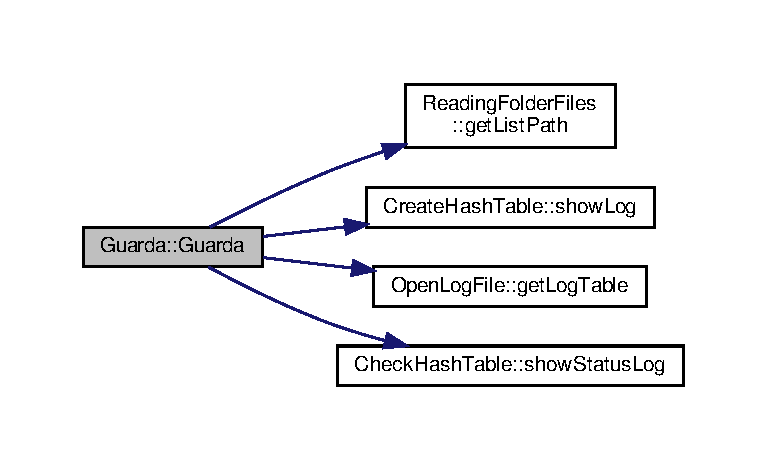
\includegraphics[width=350pt]{d9/d5b/class_guarda_a5d30e218759232802910bb3cabaddd2e_cgraph}
\end{center}
\end{figure}
\mbox{\Hypertarget{class_guarda_a296a1dd9b44b5a69e693692d5edccfe5}\label{class_guarda_a296a1dd9b44b5a69e693692d5edccfe5}} 
\index{Guarda@{Guarda}!Guarda@{Guarda}}
\index{Guarda@{Guarda}!Guarda@{Guarda}}
\subsubsection{\texorpdfstring{Guarda()}{Guarda()}\hspace{0.1cm}{\footnotesize\ttfamily [2/4]}}
{\footnotesize\ttfamily Guarda\+::\+Guarda (\begin{DoxyParamCaption}\item[{std\+::string}]{opcao,  }\item[{std\+::string}]{pasta,  }\item[{std\+::string}]{senha }\end{DoxyParamCaption})}



Construct a new \hyperlink{class_guarda}{Guarda}\+:\+: \hyperlink{class_guarda}{Guarda} object para método H\+M\+AC e sem saída em arquivo. 


\begin{DoxyParams}{Parameters}
{\em opcao} & Opção selecionada \\
\hline
{\em pasta} & Pasta a ser operada \\
\hline
{\em senha} & Senha Hmac \\
\hline
\end{DoxyParams}


Definition at line 63 of file Guarda.\+cpp.

Here is the call graph for this function\+:
\nopagebreak
\begin{figure}[H]
\begin{center}
\leavevmode
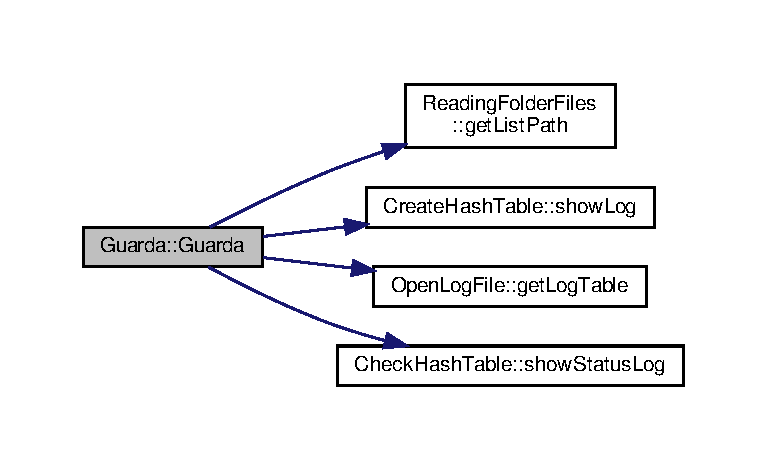
\includegraphics[width=350pt]{d9/d5b/class_guarda_a296a1dd9b44b5a69e693692d5edccfe5_cgraph}
\end{center}
\end{figure}
\mbox{\Hypertarget{class_guarda_a3a1bf11b17ec5a11a3898b2cd7a84db4}\label{class_guarda_a3a1bf11b17ec5a11a3898b2cd7a84db4}} 
\index{Guarda@{Guarda}!Guarda@{Guarda}}
\index{Guarda@{Guarda}!Guarda@{Guarda}}
\subsubsection{\texorpdfstring{Guarda()}{Guarda()}\hspace{0.1cm}{\footnotesize\ttfamily [3/4]}}
{\footnotesize\ttfamily Guarda\+::\+Guarda (\begin{DoxyParamCaption}\item[{std\+::string}]{opcao,  }\item[{std\+::string}]{pasta,  }\item[{bool}]{saida,  }\item[{std\+::string}]{destino }\end{DoxyParamCaption})}



Construct a new \hyperlink{class_guarda}{Guarda}\+:\+: \hyperlink{class_guarda}{Guarda} object para método H\+A\+SH e com saída em arquivo. 


\begin{DoxyParams}{Parameters}
{\em opcao} & Opção selecionada \\
\hline
{\em pasta} & Pasta a ser operada \\
\hline
{\em saida} & Opção de saída ativada \\
\hline
{\em destino} & Destino da saída \\
\hline
\end{DoxyParams}


Definition at line 98 of file Guarda.\+cpp.

Here is the call graph for this function\+:
\nopagebreak
\begin{figure}[H]
\begin{center}
\leavevmode
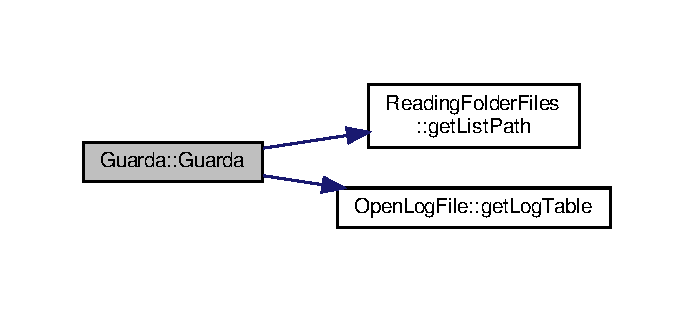
\includegraphics[width=333pt]{d9/d5b/class_guarda_a3a1bf11b17ec5a11a3898b2cd7a84db4_cgraph}
\end{center}
\end{figure}
\mbox{\Hypertarget{class_guarda_a10e2b924623ddfbbd76c3f8bb72eeaa1}\label{class_guarda_a10e2b924623ddfbbd76c3f8bb72eeaa1}} 
\index{Guarda@{Guarda}!Guarda@{Guarda}}
\index{Guarda@{Guarda}!Guarda@{Guarda}}
\subsubsection{\texorpdfstring{Guarda()}{Guarda()}\hspace{0.1cm}{\footnotesize\ttfamily [4/4]}}
{\footnotesize\ttfamily Guarda\+::\+Guarda (\begin{DoxyParamCaption}\item[{std\+::string}]{opcao,  }\item[{std\+::string}]{pasta,  }\item[{std\+::string}]{senha,  }\item[{bool}]{saida,  }\item[{std\+::string}]{destino }\end{DoxyParamCaption})}



Construct a new \hyperlink{class_guarda}{Guarda}\+:\+: \hyperlink{class_guarda}{Guarda} object para método H\+M\+AC e com saída em arquivo. 


\begin{DoxyParams}{Parameters}
{\em opcao} & Opção selecionada \\
\hline
{\em pasta} & Pasta a ser operada \\
\hline
{\em senha} & Senha Hmac \\
\hline
{\em saida} & Opção de saída ativada \\
\hline
{\em destino} & Destino da saída \\
\hline
\end{DoxyParams}


Definition at line 141 of file Guarda.\+cpp.

Here is the call graph for this function\+:
\nopagebreak
\begin{figure}[H]
\begin{center}
\leavevmode
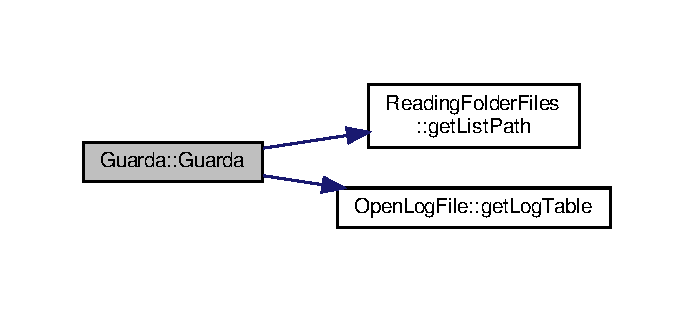
\includegraphics[width=333pt]{d9/d5b/class_guarda_a10e2b924623ddfbbd76c3f8bb72eeaa1_cgraph}
\end{center}
\end{figure}
\mbox{\Hypertarget{class_guarda_a07d37de01a671d0b698607ba872c3a76}\label{class_guarda_a07d37de01a671d0b698607ba872c3a76}} 
\index{Guarda@{Guarda}!````~Guarda@{$\sim$\+Guarda}}
\index{````~Guarda@{$\sim$\+Guarda}!Guarda@{Guarda}}
\subsubsection{\texorpdfstring{$\sim$\+Guarda()}{~Guarda()}}
{\footnotesize\ttfamily Guarda\+::$\sim$\+Guarda (\begin{DoxyParamCaption}\item[{void}]{ }\end{DoxyParamCaption})}



Destroy the \hyperlink{class_guarda}{Guarda}\+:\+: \hyperlink{class_guarda}{Guarda} object. 



Definition at line 179 of file Guarda.\+cpp.



The documentation for this class was generated from the following files\+:\begin{DoxyCompactItemize}
\item 
/home/allandemiranda/\+Documentos/\+Hash-\/\+Leva-\/\+Jeito/include/\hyperlink{_guarda_8hpp}{Guarda.\+hpp}\item 
/home/allandemiranda/\+Documentos/\+Hash-\/\+Leva-\/\+Jeito/src/\hyperlink{_guarda_8cpp}{Guarda.\+cpp}\end{DoxyCompactItemize}

\hypertarget{class_hash_file}{}\section{Hash\+File Class Reference}
\label{class_hash_file}\index{Hash\+File@{Hash\+File}}


{\ttfamily \#include $<$Hash\+File.\+hpp$>$}

\subsection*{Public Member Functions}
\begin{DoxyCompactItemize}
\item 
std\+::string \hyperlink{class_hash_file_a63590090cde4f86ec04687f7f380fb71}{get\+Hash} (void)
\begin{DoxyCompactList}\small\item\em Get the Hash object. \end{DoxyCompactList}\item 
\hyperlink{class_hash_file_abdb00953b496b5742ba036a12d0ab72e}{Hash\+File} (std\+::string)
\begin{DoxyCompactList}\small\item\em Construct a new Hash File\+:\+: Hash File object. \end{DoxyCompactList}\item 
\hyperlink{class_hash_file_afe9a013898ac44694779d413eba3b196}{Hash\+File} (std\+::string, std\+::string)
\begin{DoxyCompactList}\small\item\em Construct a new Hash File\+:\+: Hash File object. \end{DoxyCompactList}\item 
\hyperlink{class_hash_file_a88cce5bf687611a893fbf728c609f4d2}{$\sim$\+Hash\+File} (void)
\begin{DoxyCompactList}\small\item\em Destroy the Hash File\+:\+: Hash File object. \end{DoxyCompactList}\end{DoxyCompactItemize}


\subsection{Detailed Description}


Definition at line 17 of file Hash\+File.\+hpp.



\subsection{Constructor \& Destructor Documentation}
\mbox{\Hypertarget{class_hash_file_abdb00953b496b5742ba036a12d0ab72e}\label{class_hash_file_abdb00953b496b5742ba036a12d0ab72e}} 
\index{Hash\+File@{Hash\+File}!Hash\+File@{Hash\+File}}
\index{Hash\+File@{Hash\+File}!Hash\+File@{Hash\+File}}
\subsubsection{\texorpdfstring{Hash\+File()}{HashFile()}\hspace{0.1cm}{\footnotesize\ttfamily [1/2]}}
{\footnotesize\ttfamily Hash\+File\+::\+Hash\+File (\begin{DoxyParamCaption}\item[{std\+::string}]{file }\end{DoxyParamCaption})}



Construct a new Hash File\+:\+: Hash File object. 


\begin{DoxyParams}{Parameters}
{\em file} & Caminho do arquivo \\
\hline
\end{DoxyParams}


Definition at line 24 of file Hash\+File.\+cpp.

\mbox{\Hypertarget{class_hash_file_afe9a013898ac44694779d413eba3b196}\label{class_hash_file_afe9a013898ac44694779d413eba3b196}} 
\index{Hash\+File@{Hash\+File}!Hash\+File@{Hash\+File}}
\index{Hash\+File@{Hash\+File}!Hash\+File@{Hash\+File}}
\subsubsection{\texorpdfstring{Hash\+File()}{HashFile()}\hspace{0.1cm}{\footnotesize\ttfamily [2/2]}}
{\footnotesize\ttfamily Hash\+File\+::\+Hash\+File (\begin{DoxyParamCaption}\item[{std\+::string}]{file,  }\item[{std\+::string}]{key }\end{DoxyParamCaption})}



Construct a new Hash File\+:\+: Hash File object. 


\begin{DoxyParams}{Parameters}
{\em file} & Caminho do arquivo \\
\hline
{\em key} & Chave \\
\hline
\end{DoxyParams}


Definition at line 32 of file Hash\+File.\+cpp.

\mbox{\Hypertarget{class_hash_file_a88cce5bf687611a893fbf728c609f4d2}\label{class_hash_file_a88cce5bf687611a893fbf728c609f4d2}} 
\index{Hash\+File@{Hash\+File}!````~Hash\+File@{$\sim$\+Hash\+File}}
\index{````~Hash\+File@{$\sim$\+Hash\+File}!Hash\+File@{Hash\+File}}
\subsubsection{\texorpdfstring{$\sim$\+Hash\+File()}{~HashFile()}}
{\footnotesize\ttfamily Hash\+File\+::$\sim$\+Hash\+File (\begin{DoxyParamCaption}\item[{void}]{ }\end{DoxyParamCaption})}



Destroy the Hash File\+:\+: Hash File object. 



Definition at line 38 of file Hash\+File.\+cpp.



\subsection{Member Function Documentation}
\mbox{\Hypertarget{class_hash_file_a63590090cde4f86ec04687f7f380fb71}\label{class_hash_file_a63590090cde4f86ec04687f7f380fb71}} 
\index{Hash\+File@{Hash\+File}!get\+Hash@{get\+Hash}}
\index{get\+Hash@{get\+Hash}!Hash\+File@{Hash\+File}}
\subsubsection{\texorpdfstring{get\+Hash()}{getHash()}}
{\footnotesize\ttfamily std\+::string Hash\+File\+::get\+Hash (\begin{DoxyParamCaption}\item[{void}]{ }\end{DoxyParamCaption})}



Get the Hash object. 

\begin{DoxyReturn}{Returns}
std\+::string Hash 
\end{DoxyReturn}


Definition at line 45 of file Hash\+File.\+cpp.

Here is the caller graph for this function\+:
\nopagebreak
\begin{figure}[H]
\begin{center}
\leavevmode
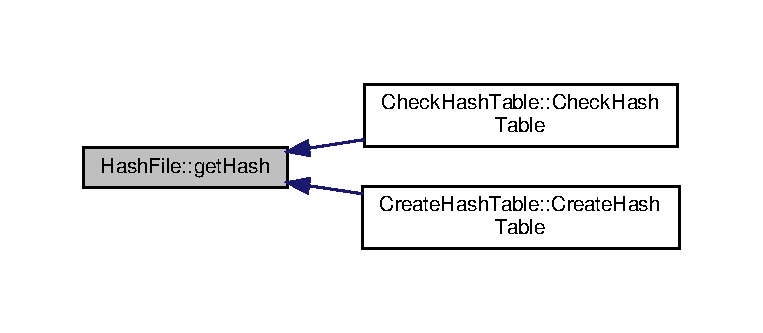
\includegraphics[width=350pt]{d0/dd4/class_hash_file_a63590090cde4f86ec04687f7f380fb71_icgraph}
\end{center}
\end{figure}


The documentation for this class was generated from the following files\+:\begin{DoxyCompactItemize}
\item 
/home/allandemiranda/\+Documentos/\+Hash-\/\+Leva-\/\+Jeito/include/\hyperlink{_hash_file_8hpp}{Hash\+File.\+hpp}\item 
/home/allandemiranda/\+Documentos/\+Hash-\/\+Leva-\/\+Jeito/src/\hyperlink{_hash_file_8cpp}{Hash\+File.\+cpp}\end{DoxyCompactItemize}

\hypertarget{class_log}{}\section{Log Class Reference}
\label{class_log}\index{Log@{Log}}


{\ttfamily \#include $<$Log.\+hpp$>$}

\subsection*{Public Member Functions}
\begin{DoxyCompactItemize}
\item 
\hyperlink{class_log_ae0979fb7a7f032fe453354c0bb204736}{Log} (std\+::string, std\+::string)
\begin{DoxyCompactList}\small\item\em Construct a new \hyperlink{class_log}{Log}\+:\+: \hyperlink{class_log}{Log} object. \end{DoxyCompactList}\item 
\hyperlink{class_log_a5c787984156efa09d466da5f2c832168}{Log} (void)
\begin{DoxyCompactList}\small\item\em Construct a new \hyperlink{class_log}{Log}\+:\+: \hyperlink{class_log}{Log} object. \end{DoxyCompactList}\item 
std\+::string \hyperlink{class_log_a9260683f85f7e9a2209cdaae19a1b582}{get\+Hash} (void)
\begin{DoxyCompactList}\small\item\em Get the Hash object. \end{DoxyCompactList}\item 
std\+::string \hyperlink{class_log_ad904745e682178df8405072499add3e2}{get\+File\+Path} (void)
\begin{DoxyCompactList}\small\item\em Get the File Path object. \end{DoxyCompactList}\item 
void \hyperlink{class_log_a15f1680044aef009232b513648a95901}{set\+Hash} (std\+::string)
\begin{DoxyCompactList}\small\item\em Set the Hash object. \end{DoxyCompactList}\item 
void \hyperlink{class_log_ab5f872112a7932749aa07c1ba649020a}{set\+File\+Path} (std\+::string)
\begin{DoxyCompactList}\small\item\em Set the File Path object. \end{DoxyCompactList}\item 
\hyperlink{class_log_ab047c1ac2053e451ff4b60c652e54353}{$\sim$\+Log} (void)
\begin{DoxyCompactList}\small\item\em Destroy the \hyperlink{class_log}{Log}\+:\+: \hyperlink{class_log}{Log} object. \end{DoxyCompactList}\end{DoxyCompactItemize}


\subsection{Detailed Description}


Definition at line 17 of file Log.\+hpp.



\subsection{Constructor \& Destructor Documentation}
\mbox{\Hypertarget{class_log_ae0979fb7a7f032fe453354c0bb204736}\label{class_log_ae0979fb7a7f032fe453354c0bb204736}} 
\index{Log@{Log}!Log@{Log}}
\index{Log@{Log}!Log@{Log}}
\subsubsection{\texorpdfstring{Log()}{Log()}\hspace{0.1cm}{\footnotesize\ttfamily [1/2]}}
{\footnotesize\ttfamily Log\+::\+Log (\begin{DoxyParamCaption}\item[{std\+::string}]{new\+\_\+hash\+\_\+md5,  }\item[{std\+::string}]{new\+\_\+file\+\_\+path }\end{DoxyParamCaption})}



Construct a new \hyperlink{class_log}{Log}\+:\+: \hyperlink{class_log}{Log} object. 


\begin{DoxyParams}{Parameters}
{\em new\+\_\+hash\+\_\+md5} & Hash para guardar \\
\hline
{\em new\+\_\+file\+\_\+path} & Caminho do arquivo guardar \\
\hline
\end{DoxyParams}


Definition at line 21 of file Log.\+cpp.

Here is the call graph for this function\+:
\nopagebreak
\begin{figure}[H]
\begin{center}
\leavevmode
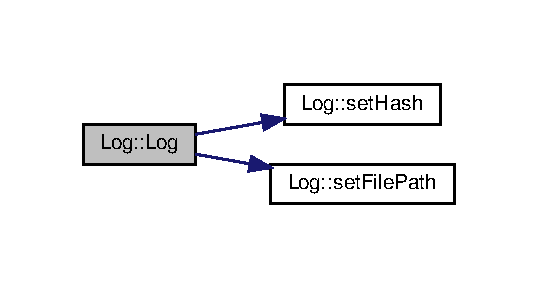
\includegraphics[width=258pt]{d6/d70/class_log_ae0979fb7a7f032fe453354c0bb204736_cgraph}
\end{center}
\end{figure}
\mbox{\Hypertarget{class_log_a5c787984156efa09d466da5f2c832168}\label{class_log_a5c787984156efa09d466da5f2c832168}} 
\index{Log@{Log}!Log@{Log}}
\index{Log@{Log}!Log@{Log}}
\subsubsection{\texorpdfstring{Log()}{Log()}\hspace{0.1cm}{\footnotesize\ttfamily [2/2]}}
{\footnotesize\ttfamily Log\+::\+Log (\begin{DoxyParamCaption}\item[{void}]{ }\end{DoxyParamCaption})}



Construct a new \hyperlink{class_log}{Log}\+:\+: \hyperlink{class_log}{Log} object. 



Definition at line 30 of file Log.\+cpp.

\mbox{\Hypertarget{class_log_ab047c1ac2053e451ff4b60c652e54353}\label{class_log_ab047c1ac2053e451ff4b60c652e54353}} 
\index{Log@{Log}!````~Log@{$\sim$\+Log}}
\index{````~Log@{$\sim$\+Log}!Log@{Log}}
\subsubsection{\texorpdfstring{$\sim$\+Log()}{~Log()}}
{\footnotesize\ttfamily Log\+::$\sim$\+Log (\begin{DoxyParamCaption}\item[{void}]{ }\end{DoxyParamCaption})}



Destroy the \hyperlink{class_log}{Log}\+:\+: \hyperlink{class_log}{Log} object. 



Definition at line 36 of file Log.\+cpp.



\subsection{Member Function Documentation}
\mbox{\Hypertarget{class_log_ad904745e682178df8405072499add3e2}\label{class_log_ad904745e682178df8405072499add3e2}} 
\index{Log@{Log}!get\+File\+Path@{get\+File\+Path}}
\index{get\+File\+Path@{get\+File\+Path}!Log@{Log}}
\subsubsection{\texorpdfstring{get\+File\+Path()}{getFilePath()}}
{\footnotesize\ttfamily std\+::string Log\+::get\+File\+Path (\begin{DoxyParamCaption}\item[{void}]{ }\end{DoxyParamCaption})}



Get the File Path object. 

\begin{DoxyReturn}{Returns}
std\+::string Caminho do arquivo guradado 
\end{DoxyReturn}


Definition at line 50 of file Log.\+cpp.

\mbox{\Hypertarget{class_log_a9260683f85f7e9a2209cdaae19a1b582}\label{class_log_a9260683f85f7e9a2209cdaae19a1b582}} 
\index{Log@{Log}!get\+Hash@{get\+Hash}}
\index{get\+Hash@{get\+Hash}!Log@{Log}}
\subsubsection{\texorpdfstring{get\+Hash()}{getHash()}}
{\footnotesize\ttfamily std\+::string Log\+::get\+Hash (\begin{DoxyParamCaption}\item[{void}]{ }\end{DoxyParamCaption})}



Get the Hash object. 

\begin{DoxyReturn}{Returns}
std\+::string Hash gurdada 
\end{DoxyReturn}


Definition at line 43 of file Log.\+cpp.

\mbox{\Hypertarget{class_log_ab5f872112a7932749aa07c1ba649020a}\label{class_log_ab5f872112a7932749aa07c1ba649020a}} 
\index{Log@{Log}!set\+File\+Path@{set\+File\+Path}}
\index{set\+File\+Path@{set\+File\+Path}!Log@{Log}}
\subsubsection{\texorpdfstring{set\+File\+Path()}{setFilePath()}}
{\footnotesize\ttfamily void Log\+::set\+File\+Path (\begin{DoxyParamCaption}\item[{std\+::string}]{new\+\_\+path }\end{DoxyParamCaption})}



Set the File Path object. 


\begin{DoxyParams}{Parameters}
{\em new\+\_\+path} & Novo caminho a quardar \\
\hline
\end{DoxyParams}


Definition at line 64 of file Log.\+cpp.

Here is the caller graph for this function\+:
\nopagebreak
\begin{figure}[H]
\begin{center}
\leavevmode
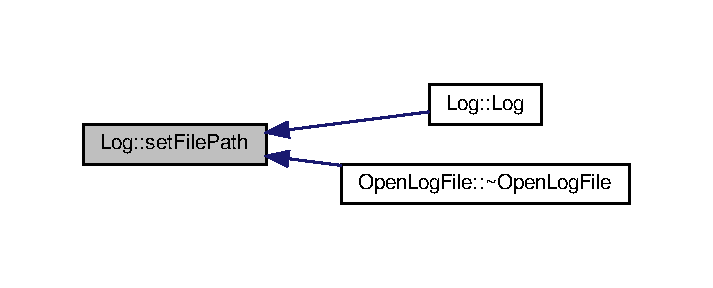
\includegraphics[width=342pt]{d6/d70/class_log_ab5f872112a7932749aa07c1ba649020a_icgraph}
\end{center}
\end{figure}
\mbox{\Hypertarget{class_log_a15f1680044aef009232b513648a95901}\label{class_log_a15f1680044aef009232b513648a95901}} 
\index{Log@{Log}!set\+Hash@{set\+Hash}}
\index{set\+Hash@{set\+Hash}!Log@{Log}}
\subsubsection{\texorpdfstring{set\+Hash()}{setHash()}}
{\footnotesize\ttfamily void Log\+::set\+Hash (\begin{DoxyParamCaption}\item[{std\+::string}]{new\+\_\+hash }\end{DoxyParamCaption})}



Set the Hash object. 


\begin{DoxyParams}{Parameters}
{\em new\+\_\+hash} & Nova hash a guradar \\
\hline
\end{DoxyParams}


Definition at line 57 of file Log.\+cpp.

Here is the caller graph for this function\+:
\nopagebreak
\begin{figure}[H]
\begin{center}
\leavevmode
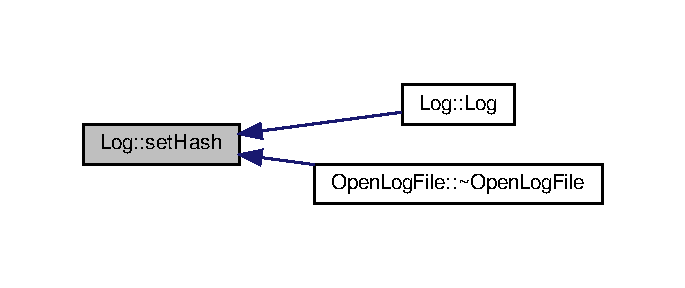
\includegraphics[width=329pt]{d6/d70/class_log_a15f1680044aef009232b513648a95901_icgraph}
\end{center}
\end{figure}


The documentation for this class was generated from the following files\+:\begin{DoxyCompactItemize}
\item 
/home/allandemiranda/\+Documentos/\+Hash-\/\+Leva-\/\+Jeito/include/\hyperlink{_log_8hpp}{Log.\+hpp}\item 
/home/allandemiranda/\+Documentos/\+Hash-\/\+Leva-\/\+Jeito/src/\hyperlink{_log_8cpp}{Log.\+cpp}\end{DoxyCompactItemize}

\hypertarget{class_open_log_file}{}\section{Open\+Log\+File Class Reference}
\label{class_open_log_file}\index{Open\+Log\+File@{Open\+Log\+File}}


{\ttfamily \#include $<$Open\+Log\+File.\+hpp$>$}

\subsection*{Public Member Functions}
\begin{DoxyCompactItemize}
\item 
std\+::vector$<$ \hyperlink{class_log}{Log} $>$ \hyperlink{class_open_log_file_ac18d5b3bc39aad3a0c2ebd761294716b}{get\+Log\+Table} (void)
\begin{DoxyCompactList}\small\item\em Get the \hyperlink{class_log}{Log} Table object. \end{DoxyCompactList}\item 
\hyperlink{class_open_log_file_a48f9d847a62a6cdc5d06b83f97023a08}{Open\+Log\+File} (std\+::string)
\begin{DoxyCompactList}\small\item\em Construct a new Open \hyperlink{class_log}{Log} File\+:\+: Open \hyperlink{class_log}{Log} File object. \end{DoxyCompactList}\item 
\hyperlink{class_open_log_file_a5583bd1705452a1c20291870539bcec0}{$\sim$\+Open\+Log\+File} (void)
\begin{DoxyCompactList}\small\item\em Destroy the Open \hyperlink{class_log}{Log} File\+:\+: Open \hyperlink{class_log}{Log} File object. \end{DoxyCompactList}\end{DoxyCompactItemize}


\subsection{Detailed Description}


Definition at line 19 of file Open\+Log\+File.\+hpp.



\subsection{Constructor \& Destructor Documentation}
\mbox{\Hypertarget{class_open_log_file_a48f9d847a62a6cdc5d06b83f97023a08}\label{class_open_log_file_a48f9d847a62a6cdc5d06b83f97023a08}} 
\index{Open\+Log\+File@{Open\+Log\+File}!Open\+Log\+File@{Open\+Log\+File}}
\index{Open\+Log\+File@{Open\+Log\+File}!Open\+Log\+File@{Open\+Log\+File}}
\subsubsection{\texorpdfstring{Open\+Log\+File()}{OpenLogFile()}}
{\footnotesize\ttfamily Open\+Log\+File\+::\+Open\+Log\+File (\begin{DoxyParamCaption}\item[{std\+::string}]{path }\end{DoxyParamCaption})}



Construct a new Open \hyperlink{class_log}{Log} File\+:\+: Open \hyperlink{class_log}{Log} File object. 


\begin{DoxyParams}{Parameters}
{\em path} & Caminho do arquivo de configuração \\
\hline
\end{DoxyParams}


Definition at line 24 of file Open\+Log\+File.\+cpp.

\mbox{\Hypertarget{class_open_log_file_a5583bd1705452a1c20291870539bcec0}\label{class_open_log_file_a5583bd1705452a1c20291870539bcec0}} 
\index{Open\+Log\+File@{Open\+Log\+File}!````~Open\+Log\+File@{$\sim$\+Open\+Log\+File}}
\index{````~Open\+Log\+File@{$\sim$\+Open\+Log\+File}!Open\+Log\+File@{Open\+Log\+File}}
\subsubsection{\texorpdfstring{$\sim$\+Open\+Log\+File()}{~OpenLogFile()}}
{\footnotesize\ttfamily Open\+Log\+File\+::$\sim$\+Open\+Log\+File (\begin{DoxyParamCaption}\item[{void}]{ }\end{DoxyParamCaption})}



Destroy the Open \hyperlink{class_log}{Log} File\+:\+: Open \hyperlink{class_log}{Log} File object. 



Definition at line 30 of file Open\+Log\+File.\+cpp.

Here is the call graph for this function\+:
\nopagebreak
\begin{figure}[H]
\begin{center}
\leavevmode
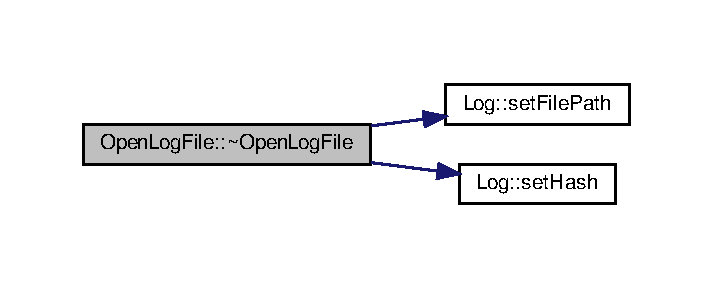
\includegraphics[width=342pt]{db/d15/class_open_log_file_a5583bd1705452a1c20291870539bcec0_cgraph}
\end{center}
\end{figure}


\subsection{Member Function Documentation}
\mbox{\Hypertarget{class_open_log_file_ac18d5b3bc39aad3a0c2ebd761294716b}\label{class_open_log_file_ac18d5b3bc39aad3a0c2ebd761294716b}} 
\index{Open\+Log\+File@{Open\+Log\+File}!get\+Log\+Table@{get\+Log\+Table}}
\index{get\+Log\+Table@{get\+Log\+Table}!Open\+Log\+File@{Open\+Log\+File}}
\subsubsection{\texorpdfstring{get\+Log\+Table()}{getLogTable()}}
{\footnotesize\ttfamily std\+::vector$<$ \hyperlink{class_log}{Log} $>$ Open\+Log\+File\+::get\+Log\+Table (\begin{DoxyParamCaption}\item[{void}]{ }\end{DoxyParamCaption})}



Get the \hyperlink{class_log}{Log} Table object. 

\begin{DoxyReturn}{Returns}
std\+::vector$<$log$>$ Dados do arquivo de configuração 
\end{DoxyReturn}


Definition at line 63 of file Open\+Log\+File.\+cpp.

Here is the caller graph for this function\+:
\nopagebreak
\begin{figure}[H]
\begin{center}
\leavevmode
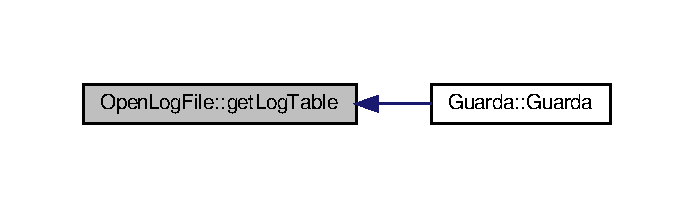
\includegraphics[width=333pt]{db/d15/class_open_log_file_ac18d5b3bc39aad3a0c2ebd761294716b_icgraph}
\end{center}
\end{figure}


The documentation for this class was generated from the following files\+:\begin{DoxyCompactItemize}
\item 
/home/allandemiranda/\+Documentos/\+Hash-\/\+Leva-\/\+Jeito/include/\hyperlink{_open_log_file_8hpp}{Open\+Log\+File.\+hpp}\item 
/home/allandemiranda/\+Documentos/\+Hash-\/\+Leva-\/\+Jeito/src/\hyperlink{_open_log_file_8cpp}{Open\+Log\+File.\+cpp}\end{DoxyCompactItemize}

\hypertarget{class_reading_folder_files}{}\section{Reading\+Folder\+Files Class Reference}
\label{class_reading_folder_files}\index{Reading\+Folder\+Files@{Reading\+Folder\+Files}}


{\ttfamily \#include $<$Reading\+Folder\+Files.\+hpp$>$}

\subsection*{Public Member Functions}
\begin{DoxyCompactItemize}
\item 
std\+::vector$<$ std\+::string $>$ \hyperlink{class_reading_folder_files_ae4eb52dbef433f34d5ccee66ebc02855}{get\+List\+Path} (void)
\begin{DoxyCompactList}\small\item\em Get the List Path object. \end{DoxyCompactList}\item 
\hyperlink{class_reading_folder_files_acd130d6bcf3f4b864e4658136c743b10}{Reading\+Folder\+Files} (std\+::string)
\begin{DoxyCompactList}\small\item\em Construct a new Reading Folder Files\+:\+: Reading Folder Files object. \end{DoxyCompactList}\item 
\hyperlink{class_reading_folder_files_a59560f57a763b2acfe78663a54f9c343}{$\sim$\+Reading\+Folder\+Files} (void)
\begin{DoxyCompactList}\small\item\em Destroy the Reading Folder Files\+:\+: Reading Folder Files object. \end{DoxyCompactList}\end{DoxyCompactItemize}


\subsection{Detailed Description}


Definition at line 19 of file Reading\+Folder\+Files.\+hpp.



\subsection{Constructor \& Destructor Documentation}
\mbox{\Hypertarget{class_reading_folder_files_acd130d6bcf3f4b864e4658136c743b10}\label{class_reading_folder_files_acd130d6bcf3f4b864e4658136c743b10}} 
\index{Reading\+Folder\+Files@{Reading\+Folder\+Files}!Reading\+Folder\+Files@{Reading\+Folder\+Files}}
\index{Reading\+Folder\+Files@{Reading\+Folder\+Files}!Reading\+Folder\+Files@{Reading\+Folder\+Files}}
\subsubsection{\texorpdfstring{Reading\+Folder\+Files()}{ReadingFolderFiles()}}
{\footnotesize\ttfamily Reading\+Folder\+Files\+::\+Reading\+Folder\+Files (\begin{DoxyParamCaption}\item[{std\+::string}]{loop\+\_\+path }\end{DoxyParamCaption})}



Construct a new Reading Folder Files\+:\+: Reading Folder Files object. 


\begin{DoxyParams}{Parameters}
{\em loop\+\_\+path} & Caminho para analisar \\
\hline
\end{DoxyParams}


Definition at line 23 of file Reading\+Folder\+Files.\+cpp.

\mbox{\Hypertarget{class_reading_folder_files_a59560f57a763b2acfe78663a54f9c343}\label{class_reading_folder_files_a59560f57a763b2acfe78663a54f9c343}} 
\index{Reading\+Folder\+Files@{Reading\+Folder\+Files}!````~Reading\+Folder\+Files@{$\sim$\+Reading\+Folder\+Files}}
\index{````~Reading\+Folder\+Files@{$\sim$\+Reading\+Folder\+Files}!Reading\+Folder\+Files@{Reading\+Folder\+Files}}
\subsubsection{\texorpdfstring{$\sim$\+Reading\+Folder\+Files()}{~ReadingFolderFiles()}}
{\footnotesize\ttfamily Reading\+Folder\+Files\+::$\sim$\+Reading\+Folder\+Files (\begin{DoxyParamCaption}\item[{void}]{ }\end{DoxyParamCaption})}



Destroy the Reading Folder Files\+:\+: Reading Folder Files object. 



Definition at line 31 of file Reading\+Folder\+Files.\+cpp.



\subsection{Member Function Documentation}
\mbox{\Hypertarget{class_reading_folder_files_ae4eb52dbef433f34d5ccee66ebc02855}\label{class_reading_folder_files_ae4eb52dbef433f34d5ccee66ebc02855}} 
\index{Reading\+Folder\+Files@{Reading\+Folder\+Files}!get\+List\+Path@{get\+List\+Path}}
\index{get\+List\+Path@{get\+List\+Path}!Reading\+Folder\+Files@{Reading\+Folder\+Files}}
\subsubsection{\texorpdfstring{get\+List\+Path()}{getListPath()}}
{\footnotesize\ttfamily std\+::vector$<$ std\+::string $>$ Reading\+Folder\+Files\+::get\+List\+Path (\begin{DoxyParamCaption}\item[{void}]{ }\end{DoxyParamCaption})}



Get the List Path object. 

\begin{DoxyReturn}{Returns}
std\+::vector$<$std\+::string$>$ Lista de caminhos de arquivos encontrados 
\end{DoxyReturn}


Definition at line 38 of file Reading\+Folder\+Files.\+cpp.

Here is the caller graph for this function\+:
\nopagebreak
\begin{figure}[H]
\begin{center}
\leavevmode
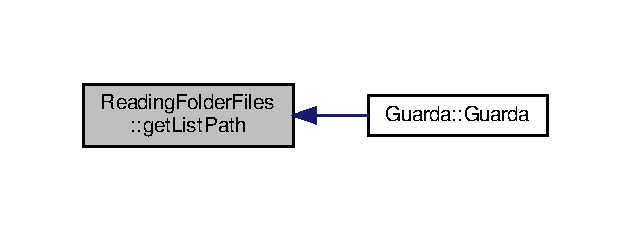
\includegraphics[width=303pt]{da/da7/class_reading_folder_files_ae4eb52dbef433f34d5ccee66ebc02855_icgraph}
\end{center}
\end{figure}


The documentation for this class was generated from the following files\+:\begin{DoxyCompactItemize}
\item 
/home/allandemiranda/\+Documentos/\+Hash-\/\+Leva-\/\+Jeito/include/\hyperlink{_reading_folder_files_8hpp}{Reading\+Folder\+Files.\+hpp}\item 
/home/allandemiranda/\+Documentos/\+Hash-\/\+Leva-\/\+Jeito/src/\hyperlink{_reading_folder_files_8cpp}{Reading\+Folder\+Files.\+cpp}\end{DoxyCompactItemize}

\hypertarget{class_report_output}{}\section{Report\+Output Class Reference}
\label{class_report_output}\index{Report\+Output@{Report\+Output}}


{\ttfamily \#include $<$Report\+Output.\+hpp$>$}

\subsection*{Public Member Functions}
\begin{DoxyCompactItemize}
\item 
\hyperlink{class_report_output_a20eb1ca7f8442fd2402f112899f6cfee}{Report\+Output} (std\+::vector$<$ \hyperlink{class_log}{Log} $>$, std\+::string)
\begin{DoxyCompactList}\small\item\em Construct a new Report Output\+:\+: Report Output object. \end{DoxyCompactList}\item 
\hyperlink{class_report_output_a6f255eea899e24768b5220ebe960ad6d}{$\sim$\+Report\+Output} (void)
\begin{DoxyCompactList}\small\item\em Destroy the Report Output\+:\+: Report Output object. \end{DoxyCompactList}\end{DoxyCompactItemize}


\subsection{Detailed Description}


Definition at line 19 of file Report\+Output.\+hpp.



\subsection{Constructor \& Destructor Documentation}
\mbox{\Hypertarget{class_report_output_a20eb1ca7f8442fd2402f112899f6cfee}\label{class_report_output_a20eb1ca7f8442fd2402f112899f6cfee}} 
\index{Report\+Output@{Report\+Output}!Report\+Output@{Report\+Output}}
\index{Report\+Output@{Report\+Output}!Report\+Output@{Report\+Output}}
\subsubsection{\texorpdfstring{Report\+Output()}{ReportOutput()}}
{\footnotesize\ttfamily Report\+Output\+::\+Report\+Output (\begin{DoxyParamCaption}\item[{std\+::vector$<$ \hyperlink{class_log}{Log} $>$}]{logs,  }\item[{std\+::string}]{path }\end{DoxyParamCaption})}



Construct a new Report Output\+:\+: Report Output object. 


\begin{DoxyParams}{Parameters}
{\em logs} & Vetor com os logs a ser salvo em um arquivo de texto \\
\hline
{\em path} & Caminho do arquivo para salvar \\
\hline
\end{DoxyParams}


Definition at line 27 of file Report\+Output.\+cpp.

\mbox{\Hypertarget{class_report_output_a6f255eea899e24768b5220ebe960ad6d}\label{class_report_output_a6f255eea899e24768b5220ebe960ad6d}} 
\index{Report\+Output@{Report\+Output}!````~Report\+Output@{$\sim$\+Report\+Output}}
\index{````~Report\+Output@{$\sim$\+Report\+Output}!Report\+Output@{Report\+Output}}
\subsubsection{\texorpdfstring{$\sim$\+Report\+Output()}{~ReportOutput()}}
{\footnotesize\ttfamily Report\+Output\+::$\sim$\+Report\+Output (\begin{DoxyParamCaption}\item[{void}]{ }\end{DoxyParamCaption})}



Destroy the Report Output\+:\+: Report Output object. 



Definition at line 35 of file Report\+Output.\+cpp.



The documentation for this class was generated from the following files\+:\begin{DoxyCompactItemize}
\item 
/home/allandemiranda/\+Documentos/\+Hash-\/\+Leva-\/\+Jeito/include/\hyperlink{_report_output_8hpp}{Report\+Output.\+hpp}\item 
/home/allandemiranda/\+Documentos/\+Hash-\/\+Leva-\/\+Jeito/src/\hyperlink{_report_output_8cpp}{Report\+Output.\+cpp}\end{DoxyCompactItemize}

\chapter{File Documentation}
\hypertarget{_check_hash_table_8hpp}{}\section{/home/allandemiranda/\+Documentos/\+Hash-\/\+Leva-\/\+Jeito/include/\+Check\+Hash\+Table.hpp File Reference}
\label{_check_hash_table_8hpp}\index{/home/allandemiranda/\+Documentos/\+Hash-\/\+Leva-\/\+Jeito/include/\+Check\+Hash\+Table.\+hpp@{/home/allandemiranda/\+Documentos/\+Hash-\/\+Leva-\/\+Jeito/include/\+Check\+Hash\+Table.\+hpp}}


Classe para comparar os arquivos com o da tabela de configuraçao.  


{\ttfamily \#include $<$string$>$}\newline
{\ttfamily \#include $<$vector$>$}\newline
{\ttfamily \#include \char`\"{}Log.\+hpp\char`\"{}}\newline
Include dependency graph for Check\+Hash\+Table.\+hpp\+:
\nopagebreak
\begin{figure}[H]
\begin{center}
\leavevmode
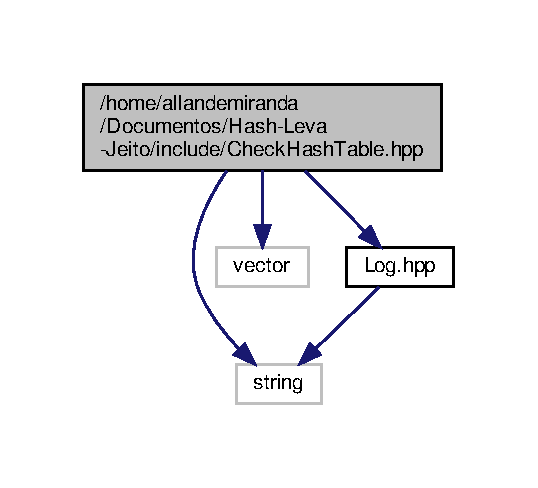
\includegraphics[width=258pt]{d7/d9a/_check_hash_table_8hpp__incl}
\end{center}
\end{figure}
This graph shows which files directly or indirectly include this file\+:
\nopagebreak
\begin{figure}[H]
\begin{center}
\leavevmode
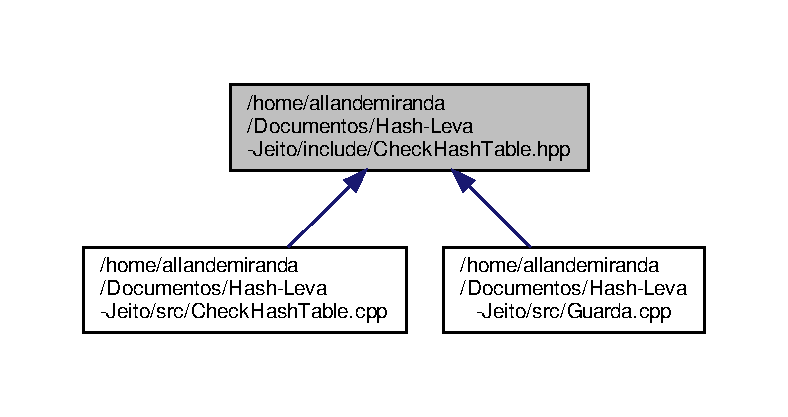
\includegraphics[width=350pt]{d6/d88/_check_hash_table_8hpp__dep__incl}
\end{center}
\end{figure}
\subsection*{Classes}
\begin{DoxyCompactItemize}
\item 
class \hyperlink{class_check_hash_table}{Check\+Hash\+Table}
\end{DoxyCompactItemize}


\subsection{Detailed Description}
Classe para comparar os arquivos com o da tabela de configuraçao. 

\begin{DoxyAuthor}{Author}
Allan de Miranda Silva (\href{mailto:allandemiranda@gmail.com}{\tt allandemiranda@gmail.\+com}) 
\end{DoxyAuthor}
\begin{DoxyVersion}{Version}
0.\+2 
\end{DoxyVersion}
\begin{DoxyDate}{Date}
25-\/09-\/2019
\end{DoxyDate}
\begin{DoxyCopyright}{Copyright}
Copyright (c) 2019 
\end{DoxyCopyright}

\hypertarget{_create_hash_table_8hpp}{}\section{/home/allandemiranda/\+Documentos/\+Hash-\/\+Leva-\/\+Jeito/include/\+Create\+Hash\+Table.hpp File Reference}
\label{_create_hash_table_8hpp}\index{/home/allandemiranda/\+Documentos/\+Hash-\/\+Leva-\/\+Jeito/include/\+Create\+Hash\+Table.\+hpp@{/home/allandemiranda/\+Documentos/\+Hash-\/\+Leva-\/\+Jeito/include/\+Create\+Hash\+Table.\+hpp}}


Classe para a criação do arquivo de configuração.  


{\ttfamily \#include $<$string$>$}\newline
{\ttfamily \#include $<$vector$>$}\newline
{\ttfamily \#include \char`\"{}Log.\+hpp\char`\"{}}\newline
Include dependency graph for Create\+Hash\+Table.\+hpp\+:
\nopagebreak
\begin{figure}[H]
\begin{center}
\leavevmode
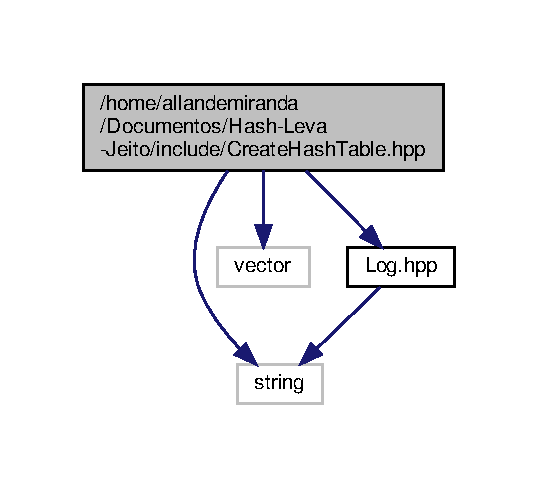
\includegraphics[width=258pt]{d8/d8c/_create_hash_table_8hpp__incl}
\end{center}
\end{figure}
This graph shows which files directly or indirectly include this file\+:
\nopagebreak
\begin{figure}[H]
\begin{center}
\leavevmode
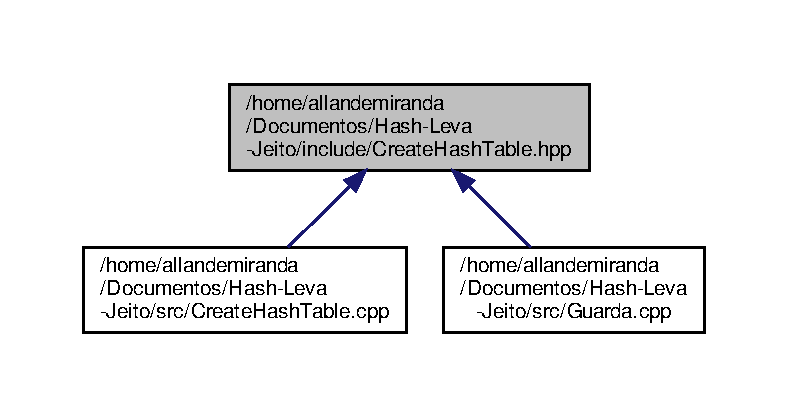
\includegraphics[width=350pt]{d5/d8f/_create_hash_table_8hpp__dep__incl}
\end{center}
\end{figure}
\subsection*{Classes}
\begin{DoxyCompactItemize}
\item 
class \hyperlink{class_create_hash_table}{Create\+Hash\+Table}
\end{DoxyCompactItemize}


\subsection{Detailed Description}
Classe para a criação do arquivo de configuração. 

\begin{DoxyAuthor}{Author}
Allan de Miranda Silva (\href{mailto:allandemiranda@gmail.com}{\tt allandemiranda@gmail.\+com}) 
\end{DoxyAuthor}
\begin{DoxyVersion}{Version}
0.\+2 
\end{DoxyVersion}
\begin{DoxyDate}{Date}
25-\/09-\/2019
\end{DoxyDate}
\begin{DoxyCopyright}{Copyright}
Copyright (c) 2019 
\end{DoxyCopyright}

\hypertarget{_guarda_8hpp}{}\section{/home/allandemiranda/\+Documentos/\+Hash-\/\+Leva-\/\+Jeito/include/\+Guarda.hpp File Reference}
\label{_guarda_8hpp}\index{/home/allandemiranda/\+Documentos/\+Hash-\/\+Leva-\/\+Jeito/include/\+Guarda.\+hpp@{/home/allandemiranda/\+Documentos/\+Hash-\/\+Leva-\/\+Jeito/include/\+Guarda.\+hpp}}


Classe de controle.  


{\ttfamily \#include $<$string$>$}\newline
Include dependency graph for Guarda.\+hpp\+:
\nopagebreak
\begin{figure}[H]
\begin{center}
\leavevmode
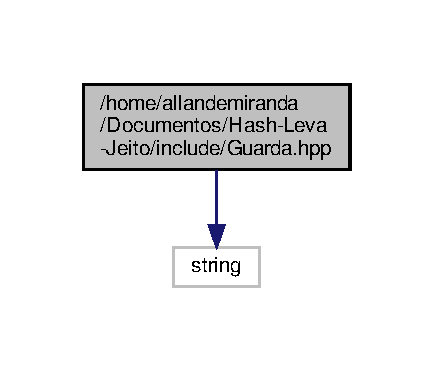
\includegraphics[width=208pt]{d8/dff/_guarda_8hpp__incl}
\end{center}
\end{figure}
This graph shows which files directly or indirectly include this file\+:
\nopagebreak
\begin{figure}[H]
\begin{center}
\leavevmode
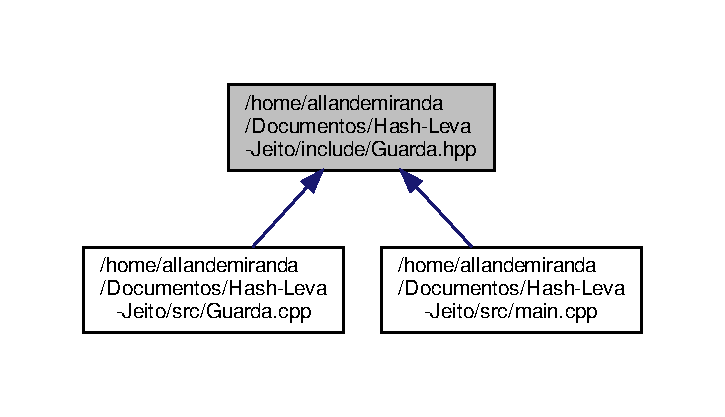
\includegraphics[width=348pt]{db/d2d/_guarda_8hpp__dep__incl}
\end{center}
\end{figure}
\subsection*{Classes}
\begin{DoxyCompactItemize}
\item 
class \hyperlink{class_guarda}{Guarda}
\end{DoxyCompactItemize}


\subsection{Detailed Description}
Classe de controle. 

\begin{DoxyAuthor}{Author}
Allan de Miranda Silva (\href{mailto:allandemiranda@gmail.com}{\tt allandemiranda@gmail.\+com}) 
\end{DoxyAuthor}
\begin{DoxyVersion}{Version}
0.\+2 
\end{DoxyVersion}
\begin{DoxyDate}{Date}
25-\/09-\/2019
\end{DoxyDate}
\begin{DoxyCopyright}{Copyright}
Copyright (c) 2019 
\end{DoxyCopyright}

\hypertarget{_hash_file_8hpp}{}\section{/home/allandemiranda/\+Documentos/\+Hash-\/\+Leva-\/\+Jeito/include/\+Hash\+File.hpp File Reference}
\label{_hash_file_8hpp}\index{/home/allandemiranda/\+Documentos/\+Hash-\/\+Leva-\/\+Jeito/include/\+Hash\+File.\+hpp@{/home/allandemiranda/\+Documentos/\+Hash-\/\+Leva-\/\+Jeito/include/\+Hash\+File.\+hpp}}


Classe que cria a hash para o arquivo solicitado.  


{\ttfamily \#include $<$string$>$}\newline
Include dependency graph for Hash\+File.\+hpp\+:
\nopagebreak
\begin{figure}[H]
\begin{center}
\leavevmode
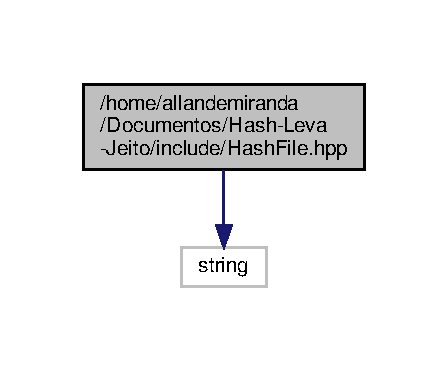
\includegraphics[width=215pt]{de/d6e/_hash_file_8hpp__incl}
\end{center}
\end{figure}
This graph shows which files directly or indirectly include this file\+:
\nopagebreak
\begin{figure}[H]
\begin{center}
\leavevmode
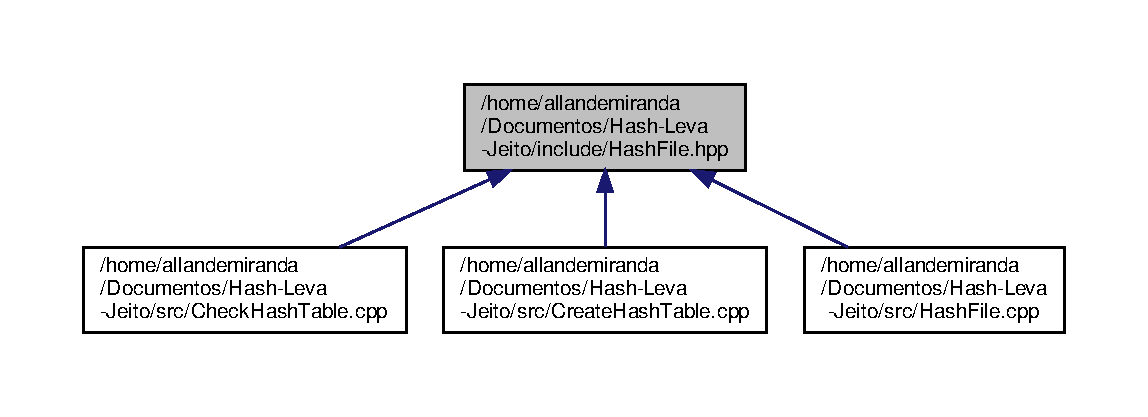
\includegraphics[width=350pt]{d0/d38/_hash_file_8hpp__dep__incl}
\end{center}
\end{figure}
\subsection*{Classes}
\begin{DoxyCompactItemize}
\item 
class \hyperlink{class_hash_file}{Hash\+File}
\end{DoxyCompactItemize}


\subsection{Detailed Description}
Classe que cria a hash para o arquivo solicitado. 

\begin{DoxyAuthor}{Author}
Allan de Miranda Silva (\href{mailto:allandemiranda@gmail.com}{\tt allandemiranda@gmail.\+com}) 
\end{DoxyAuthor}
\begin{DoxyVersion}{Version}
0.\+1 
\end{DoxyVersion}
\begin{DoxyDate}{Date}
25-\/09-\/2019
\end{DoxyDate}
\begin{DoxyCopyright}{Copyright}
Copyright (c) 2019 
\end{DoxyCopyright}

\hypertarget{_log_8hpp}{}\section{/home/allandemiranda/\+Documentos/\+Hash-\/\+Leva-\/\+Jeito/include/\+Log.hpp File Reference}
\label{_log_8hpp}\index{/home/allandemiranda/\+Documentos/\+Hash-\/\+Leva-\/\+Jeito/include/\+Log.\+hpp@{/home/allandemiranda/\+Documentos/\+Hash-\/\+Leva-\/\+Jeito/include/\+Log.\+hpp}}


Classe para gerenciar o modelo de logs.  


{\ttfamily \#include $<$string$>$}\newline
Include dependency graph for Log.\+hpp\+:
\nopagebreak
\begin{figure}[H]
\begin{center}
\leavevmode
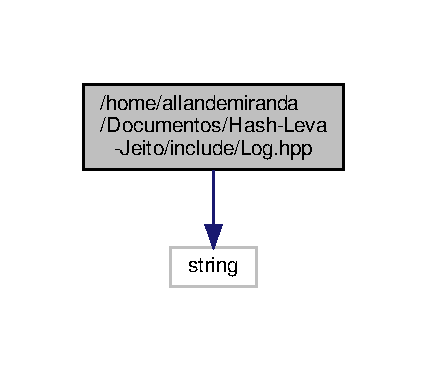
\includegraphics[width=205pt]{d7/d5b/_log_8hpp__incl}
\end{center}
\end{figure}
This graph shows which files directly or indirectly include this file\+:
\nopagebreak
\begin{figure}[H]
\begin{center}
\leavevmode
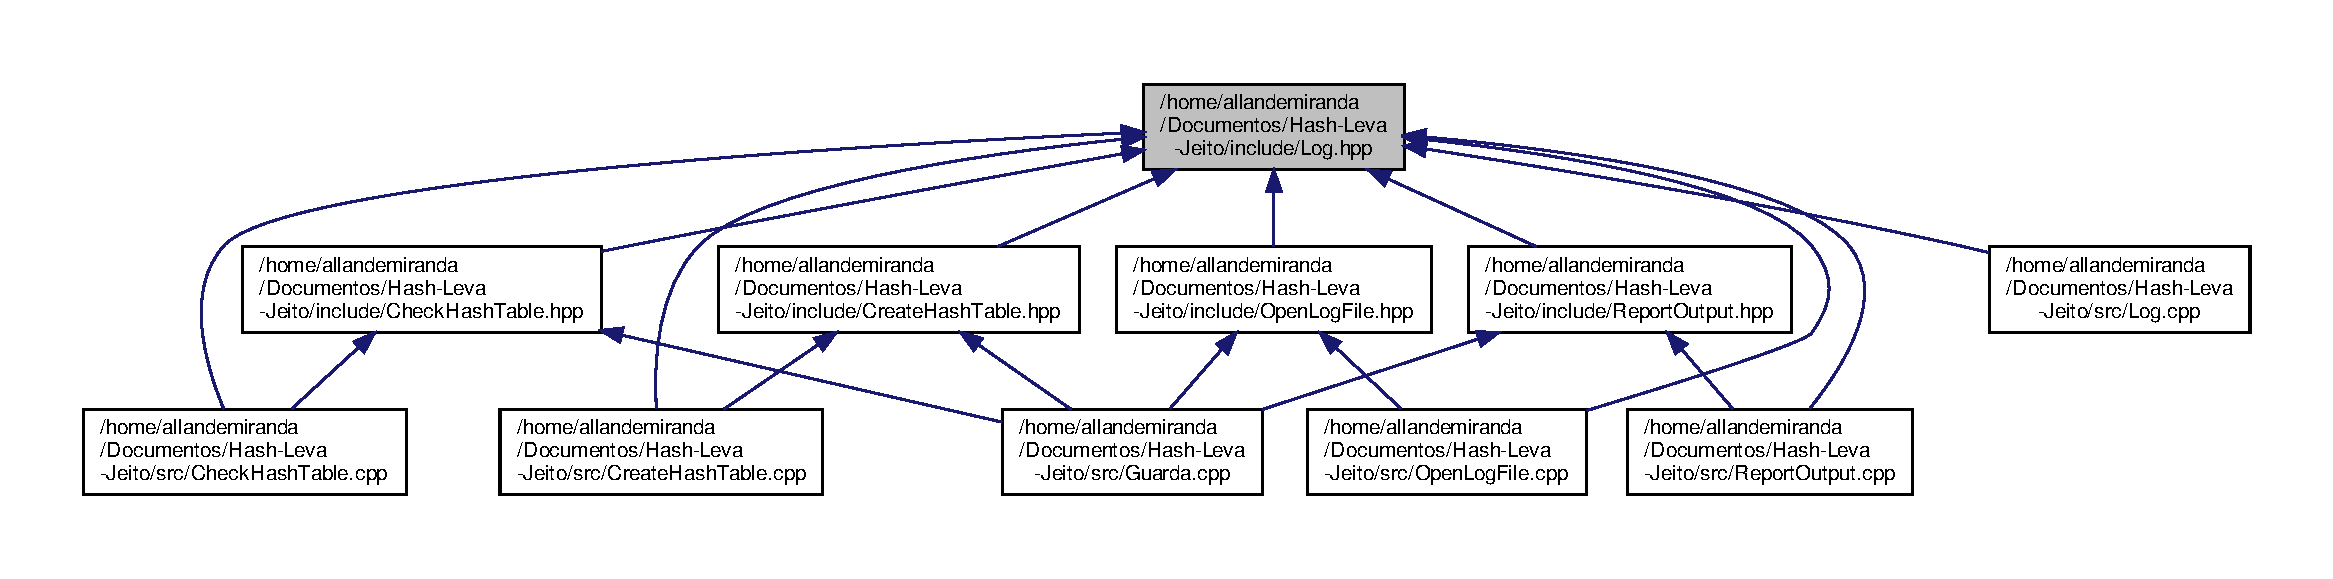
\includegraphics[width=350pt]{d3/d58/_log_8hpp__dep__incl}
\end{center}
\end{figure}
\subsection*{Classes}
\begin{DoxyCompactItemize}
\item 
class \hyperlink{class_log}{Log}
\end{DoxyCompactItemize}


\subsection{Detailed Description}
Classe para gerenciar o modelo de logs. 

\begin{DoxyAuthor}{Author}
Allan de Miranda Silva (\href{mailto:allandemiranda@gmail.com}{\tt allandemiranda@gmail.\+com}) 
\end{DoxyAuthor}
\begin{DoxyVersion}{Version}
0.\+1 
\end{DoxyVersion}
\begin{DoxyDate}{Date}
25-\/09-\/2019
\end{DoxyDate}
\begin{DoxyCopyright}{Copyright}
Copyright (c) 2019 
\end{DoxyCopyright}

\hypertarget{_open_log_file_8hpp}{}\section{/home/allandemiranda/\+Documentos/\+Hash-\/\+Leva-\/\+Jeito/include/\+Open\+Log\+File.hpp File Reference}
\label{_open_log_file_8hpp}\index{/home/allandemiranda/\+Documentos/\+Hash-\/\+Leva-\/\+Jeito/include/\+Open\+Log\+File.\+hpp@{/home/allandemiranda/\+Documentos/\+Hash-\/\+Leva-\/\+Jeito/include/\+Open\+Log\+File.\+hpp}}


Classe para abrir arquivos de log de acordo com o padrão solicitado.  


{\ttfamily \#include $<$string$>$}\newline
{\ttfamily \#include $<$vector$>$}\newline
{\ttfamily \#include \char`\"{}Log.\+hpp\char`\"{}}\newline
Include dependency graph for Open\+Log\+File.\+hpp\+:
\nopagebreak
\begin{figure}[H]
\begin{center}
\leavevmode
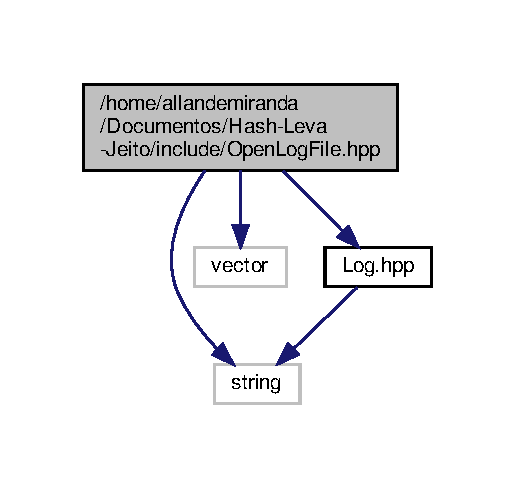
\includegraphics[width=247pt]{dc/df6/_open_log_file_8hpp__incl}
\end{center}
\end{figure}
This graph shows which files directly or indirectly include this file\+:
\nopagebreak
\begin{figure}[H]
\begin{center}
\leavevmode
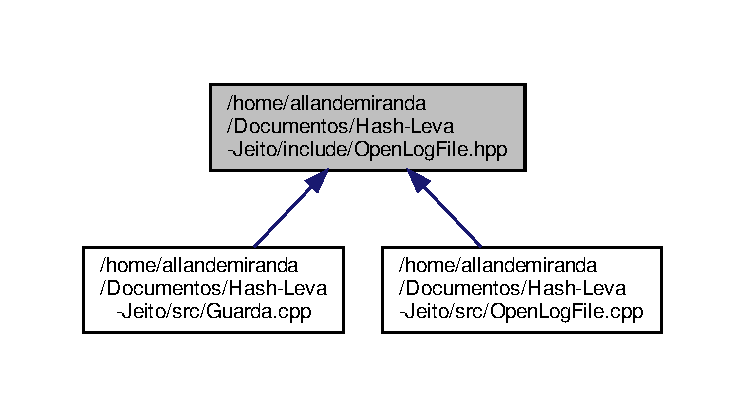
\includegraphics[width=350pt]{de/d33/_open_log_file_8hpp__dep__incl}
\end{center}
\end{figure}
\subsection*{Classes}
\begin{DoxyCompactItemize}
\item 
class \hyperlink{class_open_log_file}{Open\+Log\+File}
\end{DoxyCompactItemize}


\subsection{Detailed Description}
Classe para abrir arquivos de log de acordo com o padrão solicitado. 

\begin{DoxyAuthor}{Author}
Allan de Miranda Silva (\href{mailto:allandemiranda@gmail.com}{\tt allandemiranda@gmail.\+com}) 
\end{DoxyAuthor}
\begin{DoxyVersion}{Version}
0.\+1 
\end{DoxyVersion}
\begin{DoxyDate}{Date}
25-\/09-\/2019
\end{DoxyDate}
\begin{DoxyCopyright}{Copyright}
Copyright (c) 2019 
\end{DoxyCopyright}

\hypertarget{_reading_folder_files_8hpp}{}\section{/home/allandemiranda/\+Documentos/\+Hash-\/\+Leva-\/\+Jeito/include/\+Reading\+Folder\+Files.hpp File Reference}
\label{_reading_folder_files_8hpp}\index{/home/allandemiranda/\+Documentos/\+Hash-\/\+Leva-\/\+Jeito/include/\+Reading\+Folder\+Files.\+hpp@{/home/allandemiranda/\+Documentos/\+Hash-\/\+Leva-\/\+Jeito/include/\+Reading\+Folder\+Files.\+hpp}}


Classe para gerenciar a leitura de todos os arquivos de todas as pastas.  


{\ttfamily \#include $<$string$>$}\newline
{\ttfamily \#include $<$vector$>$}\newline
Include dependency graph for Reading\+Folder\+Files.\+hpp\+:
\nopagebreak
\begin{figure}[H]
\begin{center}
\leavevmode
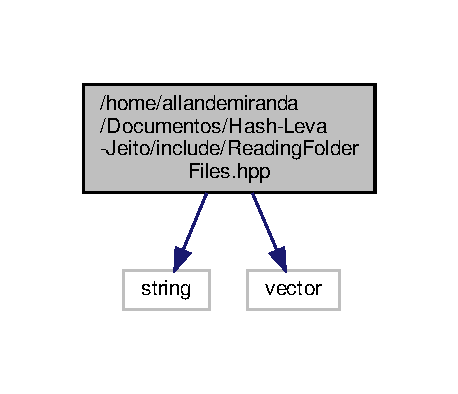
\includegraphics[width=220pt]{d7/d0d/_reading_folder_files_8hpp__incl}
\end{center}
\end{figure}
This graph shows which files directly or indirectly include this file\+:
\nopagebreak
\begin{figure}[H]
\begin{center}
\leavevmode
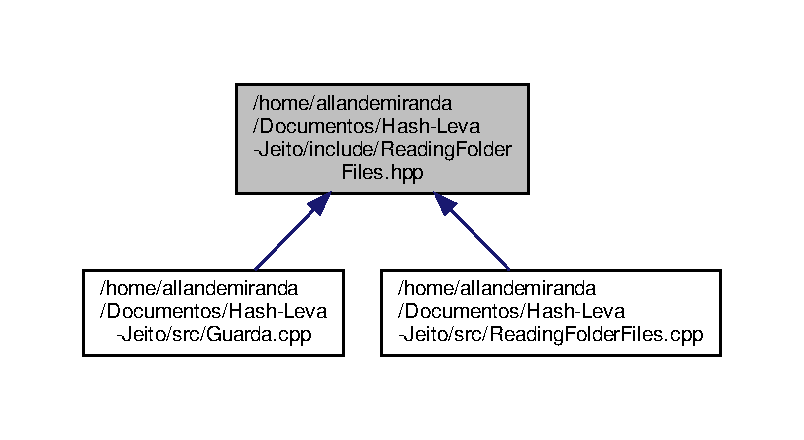
\includegraphics[width=350pt]{d0/d1e/_reading_folder_files_8hpp__dep__incl}
\end{center}
\end{figure}
\subsection*{Classes}
\begin{DoxyCompactItemize}
\item 
class \hyperlink{class_reading_folder_files}{Reading\+Folder\+Files}
\end{DoxyCompactItemize}


\subsection{Detailed Description}
Classe para gerenciar a leitura de todos os arquivos de todas as pastas. 

\begin{DoxyAuthor}{Author}
Allan de Miranda Silva (\href{mailto:allandemiranda@gmail.com}{\tt allandemiranda@gmail.\+com}) 
\end{DoxyAuthor}
\begin{DoxyVersion}{Version}
0.\+1 
\end{DoxyVersion}
\begin{DoxyDate}{Date}
25-\/09-\/2019
\end{DoxyDate}
\begin{DoxyCopyright}{Copyright}
Copyright (c) 2019 
\end{DoxyCopyright}

\hypertarget{_report_output_8hpp}{}\section{/home/allandemiranda/\+Documentos/\+Hash-\/\+Leva-\/\+Jeito/include/\+Report\+Output.hpp File Reference}
\label{_report_output_8hpp}\index{/home/allandemiranda/\+Documentos/\+Hash-\/\+Leva-\/\+Jeito/include/\+Report\+Output.\+hpp@{/home/allandemiranda/\+Documentos/\+Hash-\/\+Leva-\/\+Jeito/include/\+Report\+Output.\+hpp}}


Classe para gerenciar saída de arquivo de log.  


{\ttfamily \#include $<$string$>$}\newline
{\ttfamily \#include $<$vector$>$}\newline
{\ttfamily \#include \char`\"{}Log.\+hpp\char`\"{}}\newline
Include dependency graph for Report\+Output.\+hpp\+:
\nopagebreak
\begin{figure}[H]
\begin{center}
\leavevmode
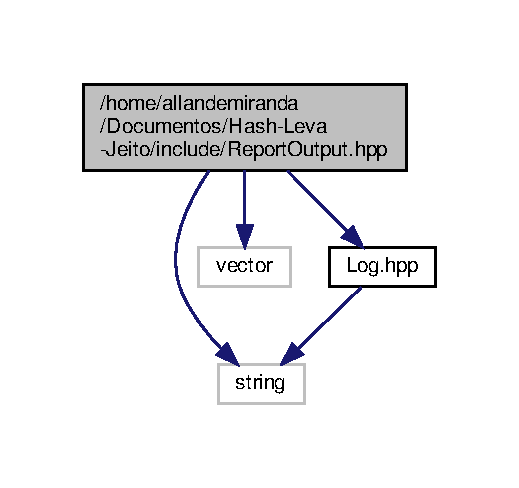
\includegraphics[width=249pt]{db/d69/_report_output_8hpp__incl}
\end{center}
\end{figure}
This graph shows which files directly or indirectly include this file\+:
\nopagebreak
\begin{figure}[H]
\begin{center}
\leavevmode
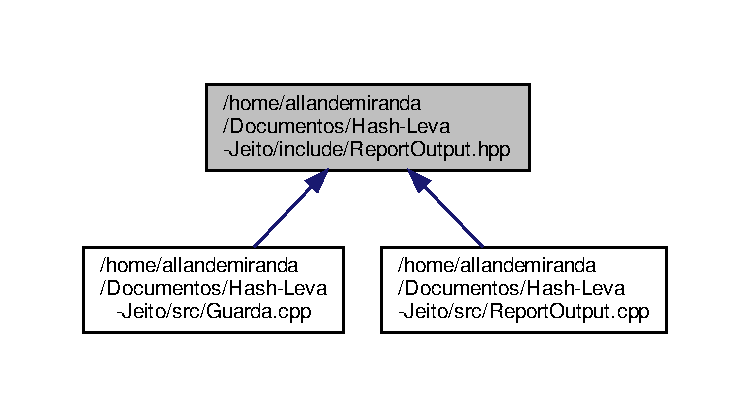
\includegraphics[width=350pt]{d2/d80/_report_output_8hpp__dep__incl}
\end{center}
\end{figure}
\subsection*{Classes}
\begin{DoxyCompactItemize}
\item 
class \hyperlink{class_report_output}{Report\+Output}
\end{DoxyCompactItemize}


\subsection{Detailed Description}
Classe para gerenciar saída de arquivo de log. 

\begin{DoxyAuthor}{Author}
Allan de Miranda Silva (\href{mailto:allandemiranda@gmail.com}{\tt allandemiranda@gmail.\+com}) 
\end{DoxyAuthor}
\begin{DoxyVersion}{Version}
0.\+1 
\end{DoxyVersion}
\begin{DoxyDate}{Date}
25-\/09-\/2019
\end{DoxyDate}
\begin{DoxyCopyright}{Copyright}
Copyright (c) 2019 
\end{DoxyCopyright}

\hypertarget{_r_e_a_d_m_e_8md}{}\section{/home/allandemiranda/\+Documentos/\+Hash-\/\+Leva-\/\+Jeito/\+R\+E\+A\+D\+ME.md File Reference}
\label{_r_e_a_d_m_e_8md}\index{/home/allandemiranda/\+Documentos/\+Hash-\/\+Leva-\/\+Jeito/\+R\+E\+A\+D\+M\+E.\+md@{/home/allandemiranda/\+Documentos/\+Hash-\/\+Leva-\/\+Jeito/\+R\+E\+A\+D\+M\+E.\+md}}

\hypertarget{_check_hash_table_8cpp}{}\section{/home/allandemiranda/\+Documentos/\+Hash-\/\+Leva-\/\+Jeito/src/\+Check\+Hash\+Table.cpp File Reference}
\label{_check_hash_table_8cpp}\index{/home/allandemiranda/\+Documentos/\+Hash-\/\+Leva-\/\+Jeito/src/\+Check\+Hash\+Table.\+cpp@{/home/allandemiranda/\+Documentos/\+Hash-\/\+Leva-\/\+Jeito/src/\+Check\+Hash\+Table.\+cpp}}


Metodos da classe \hyperlink{class_check_hash_table}{Check\+Hash\+Table}.  


{\ttfamily \#include \char`\"{}Check\+Hash\+Table.\+hpp\char`\"{}}\newline
{\ttfamily \#include $<$iomanip$>$}\newline
{\ttfamily \#include $<$iostream$>$}\newline
{\ttfamily \#include $<$string$>$}\newline
{\ttfamily \#include $<$vector$>$}\newline
{\ttfamily \#include \char`\"{}Hash\+File.\+hpp\char`\"{}}\newline
{\ttfamily \#include \char`\"{}Log.\+hpp\char`\"{}}\newline
Include dependency graph for Check\+Hash\+Table.\+cpp\+:
\nopagebreak
\begin{figure}[H]
\begin{center}
\leavevmode
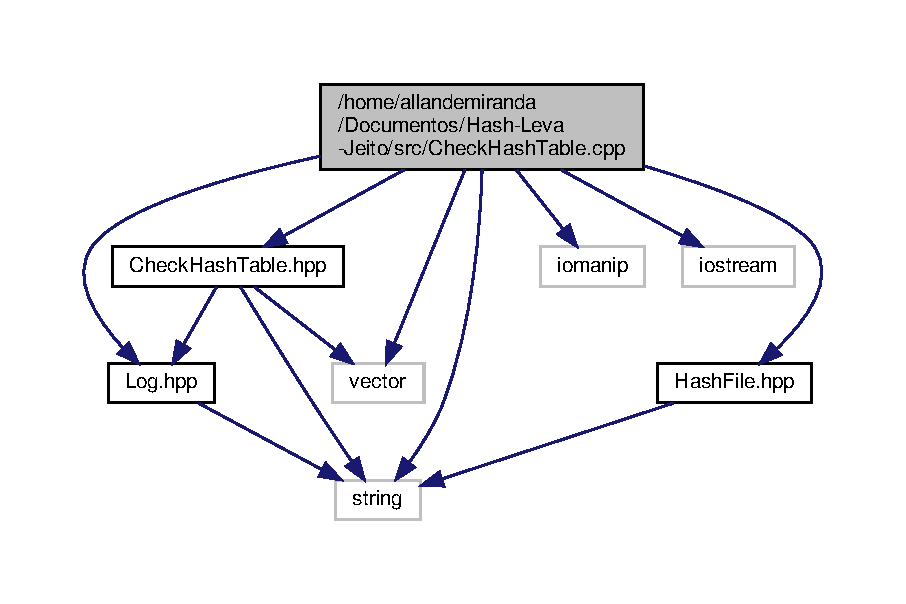
\includegraphics[width=350pt]{d5/d24/_check_hash_table_8cpp__incl}
\end{center}
\end{figure}


\subsection{Detailed Description}
Metodos da classe \hyperlink{class_check_hash_table}{Check\+Hash\+Table}. 

\begin{DoxyAuthor}{Author}
Allan de Miranda Silva (\href{mailto:allandemiranda@gmail.com}{\tt allandemiranda@gmail.\+com}) 
\end{DoxyAuthor}
\begin{DoxyVersion}{Version}
0.\+2 
\end{DoxyVersion}
\begin{DoxyDate}{Date}
25-\/09-\/2019
\end{DoxyDate}
\begin{DoxyCopyright}{Copyright}
Copyright (c) 2019 
\end{DoxyCopyright}

\hypertarget{_create_hash_table_8cpp}{}\section{/home/allandemiranda/\+Documentos/\+Hash-\/\+Leva-\/\+Jeito/src/\+Create\+Hash\+Table.cpp File Reference}
\label{_create_hash_table_8cpp}\index{/home/allandemiranda/\+Documentos/\+Hash-\/\+Leva-\/\+Jeito/src/\+Create\+Hash\+Table.\+cpp@{/home/allandemiranda/\+Documentos/\+Hash-\/\+Leva-\/\+Jeito/src/\+Create\+Hash\+Table.\+cpp}}


Métodos para classe \hyperlink{class_create_hash_table}{Create\+Hash\+Table}.  


{\ttfamily \#include \char`\"{}Create\+Hash\+Table.\+hpp\char`\"{}}\newline
{\ttfamily \#include $<$iomanip$>$}\newline
{\ttfamily \#include $<$iostream$>$}\newline
{\ttfamily \#include $<$string$>$}\newline
{\ttfamily \#include $<$vector$>$}\newline
{\ttfamily \#include \char`\"{}Hash\+File.\+hpp\char`\"{}}\newline
{\ttfamily \#include \char`\"{}Log.\+hpp\char`\"{}}\newline
Include dependency graph for Create\+Hash\+Table.\+cpp\+:
\nopagebreak
\begin{figure}[H]
\begin{center}
\leavevmode
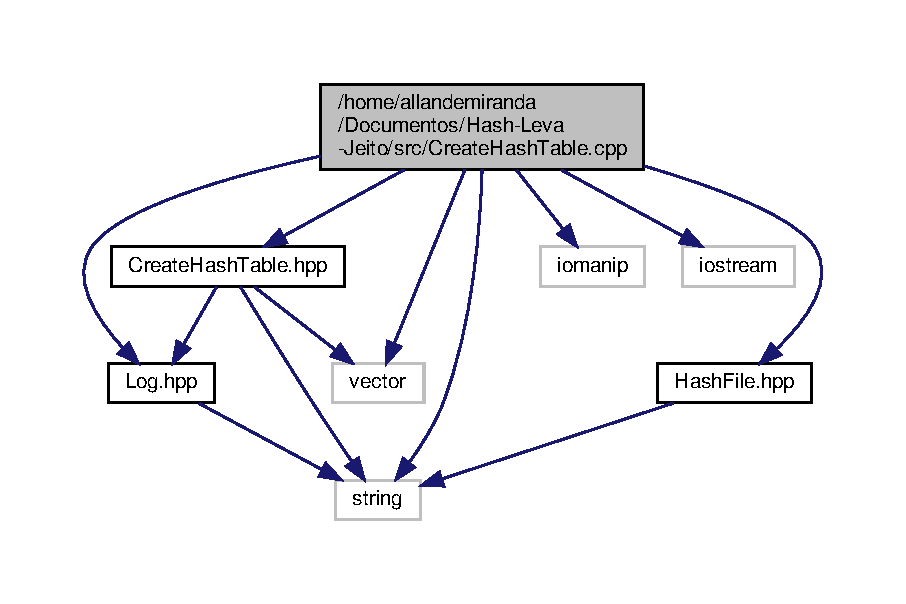
\includegraphics[width=350pt]{db/dd0/_create_hash_table_8cpp__incl}
\end{center}
\end{figure}


\subsection{Detailed Description}
Métodos para classe \hyperlink{class_create_hash_table}{Create\+Hash\+Table}. 

\begin{DoxyAuthor}{Author}
Allan de Miranda Silva (\href{mailto:allandemiranda@gmail.com}{\tt allandemiranda@gmail.\+com}) 
\end{DoxyAuthor}
\begin{DoxyVersion}{Version}
0.\+2 
\end{DoxyVersion}
\begin{DoxyDate}{Date}
25-\/09-\/2019
\end{DoxyDate}
\begin{DoxyCopyright}{Copyright}
Copyright (c) 2019 
\end{DoxyCopyright}

\hypertarget{_guarda_8cpp}{}\section{/home/allandemiranda/\+Documentos/\+Hash-\/\+Leva-\/\+Jeito/src/\+Guarda.cpp File Reference}
\label{_guarda_8cpp}\index{/home/allandemiranda/\+Documentos/\+Hash-\/\+Leva-\/\+Jeito/src/\+Guarda.\+cpp@{/home/allandemiranda/\+Documentos/\+Hash-\/\+Leva-\/\+Jeito/src/\+Guarda.\+cpp}}


Métodos para classe \hyperlink{class_guarda}{Guarda}.  


{\ttfamily \#include \char`\"{}Guarda.\+hpp\char`\"{}}\newline
{\ttfamily \#include $<$cstring$>$}\newline
{\ttfamily \#include $<$iostream$>$}\newline
{\ttfamily \#include $<$string$>$}\newline
{\ttfamily \#include \char`\"{}Check\+Hash\+Table.\+hpp\char`\"{}}\newline
{\ttfamily \#include \char`\"{}Create\+Hash\+Table.\+hpp\char`\"{}}\newline
{\ttfamily \#include \char`\"{}Open\+Log\+File.\+hpp\char`\"{}}\newline
{\ttfamily \#include \char`\"{}Reading\+Folder\+Files.\+hpp\char`\"{}}\newline
{\ttfamily \#include \char`\"{}Report\+Output.\+hpp\char`\"{}}\newline
Include dependency graph for Guarda.\+cpp\+:
\nopagebreak
\begin{figure}[H]
\begin{center}
\leavevmode
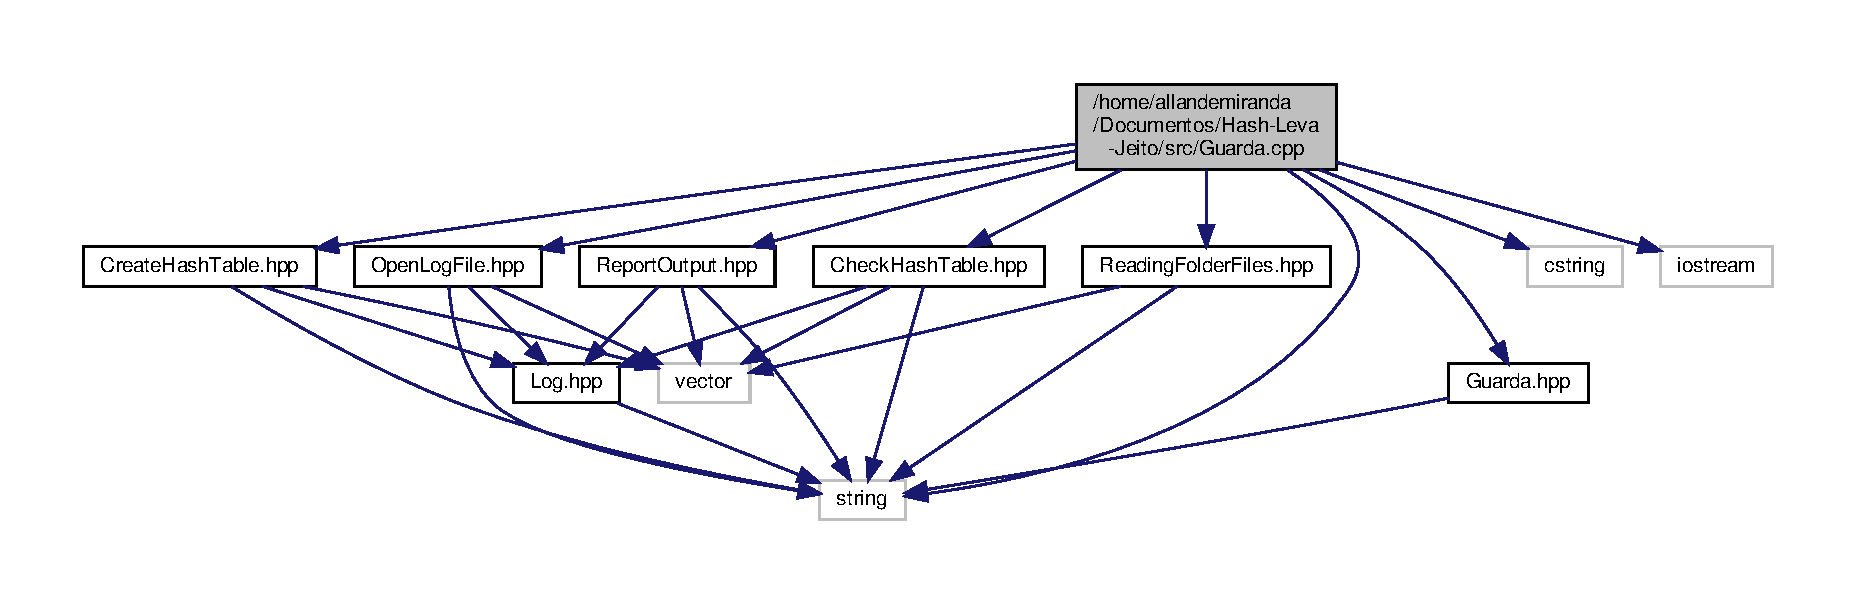
\includegraphics[width=350pt]{d4/d51/_guarda_8cpp__incl}
\end{center}
\end{figure}


\subsection{Detailed Description}
Métodos para classe \hyperlink{class_guarda}{Guarda}. 

\begin{DoxyAuthor}{Author}
Allan de Miranda Silva (\href{mailto:allandemiranda@gmail.com}{\tt allandemiranda@gmail.\+com}) 
\end{DoxyAuthor}
\begin{DoxyVersion}{Version}
0.\+2 
\end{DoxyVersion}
\begin{DoxyDate}{Date}
25-\/09-\/2019
\end{DoxyDate}
\begin{DoxyCopyright}{Copyright}
Copyright (c) 2019 
\end{DoxyCopyright}

\hypertarget{_hash_file_8cpp}{}\section{/home/allandemiranda/\+Documentos/\+Hash-\/\+Leva-\/\+Jeito/src/\+Hash\+File.cpp File Reference}
\label{_hash_file_8cpp}\index{/home/allandemiranda/\+Documentos/\+Hash-\/\+Leva-\/\+Jeito/src/\+Hash\+File.\+cpp@{/home/allandemiranda/\+Documentos/\+Hash-\/\+Leva-\/\+Jeito/src/\+Hash\+File.\+cpp}}


Métodos para classe \hyperlink{class_hash_file}{Hash\+File}.  


{\ttfamily \#include \char`\"{}Hash\+File.\+hpp\char`\"{}}\newline
{\ttfamily \#include $<$openssl/hmac.\+h$>$}\newline
{\ttfamily \#include $<$openssl/md5.\+h$>$}\newline
{\ttfamily \#include $<$boost/iostreams/device/mapped\+\_\+file.\+hpp$>$}\newline
{\ttfamily \#include $<$iomanip$>$}\newline
{\ttfamily \#include $<$sstream$>$}\newline
Include dependency graph for Hash\+File.\+cpp\+:
\nopagebreak
\begin{figure}[H]
\begin{center}
\leavevmode
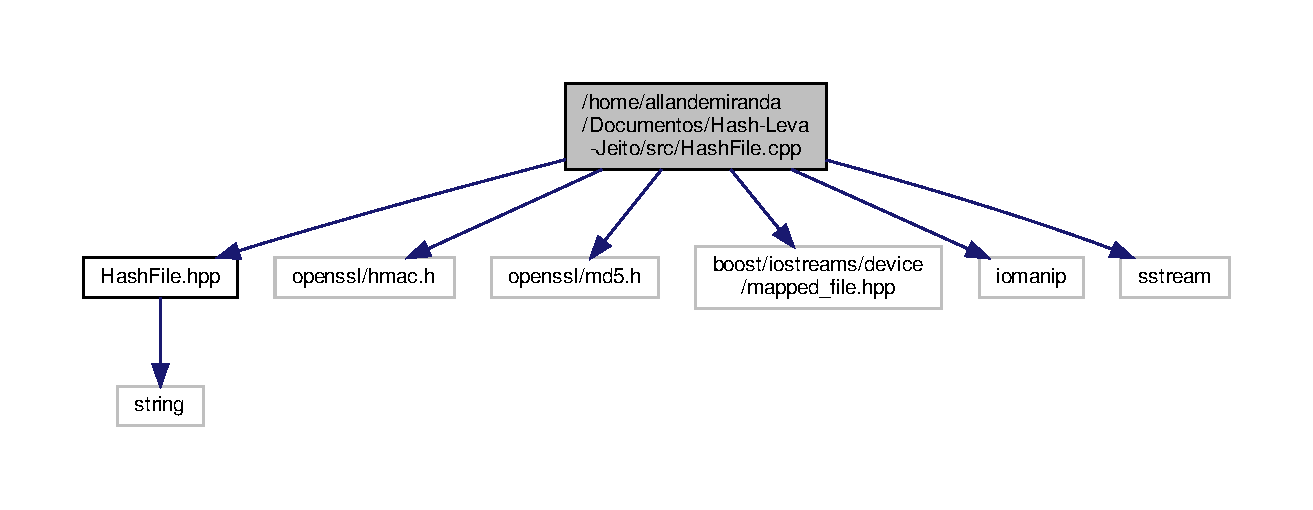
\includegraphics[width=350pt]{d8/de8/_hash_file_8cpp__incl}
\end{center}
\end{figure}


\subsection{Detailed Description}
Métodos para classe \hyperlink{class_hash_file}{Hash\+File}. 

\begin{DoxyAuthor}{Author}
Allan de Miranda Silva (\href{mailto:allandemiranda@gmail.com}{\tt allandemiranda@gmail.\+com}) 
\end{DoxyAuthor}
\begin{DoxyVersion}{Version}
0.\+1 
\end{DoxyVersion}
\begin{DoxyDate}{Date}
25-\/09-\/2019
\end{DoxyDate}
\begin{DoxyCopyright}{Copyright}
Copyright (c) 2019 
\end{DoxyCopyright}

\hypertarget{_log_8cpp}{}\section{/home/allandemiranda/\+Documentos/\+Hash-\/\+Leva-\/\+Jeito/src/\+Log.cpp File Reference}
\label{_log_8cpp}\index{/home/allandemiranda/\+Documentos/\+Hash-\/\+Leva-\/\+Jeito/src/\+Log.\+cpp@{/home/allandemiranda/\+Documentos/\+Hash-\/\+Leva-\/\+Jeito/src/\+Log.\+cpp}}


Métodos da classe \hyperlink{class_log}{Log}.  


{\ttfamily \#include \char`\"{}Log.\+hpp\char`\"{}}\newline
{\ttfamily \#include $<$string$>$}\newline
Include dependency graph for Log.\+cpp\+:
\nopagebreak
\begin{figure}[H]
\begin{center}
\leavevmode
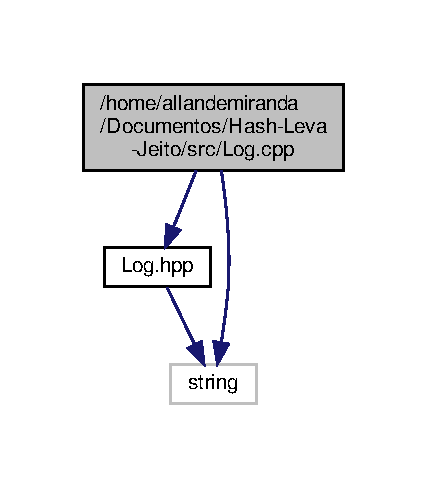
\includegraphics[width=205pt]{da/d68/_log_8cpp__incl}
\end{center}
\end{figure}


\subsection{Detailed Description}
Métodos da classe \hyperlink{class_log}{Log}. 

\begin{DoxyAuthor}{Author}
Allan de Miranda Silva (\href{mailto:allandemiranda@gmail.com}{\tt allandemiranda@gmail.\+com}) 
\end{DoxyAuthor}
\begin{DoxyVersion}{Version}
0.\+1 
\end{DoxyVersion}
\begin{DoxyDate}{Date}
25-\/09-\/2019
\end{DoxyDate}
\begin{DoxyCopyright}{Copyright}
Copyright (c) 2019 
\end{DoxyCopyright}

\hypertarget{main_8cpp}{}\section{/home/allandemiranda/\+Documentos/\+Hash-\/\+Leva-\/\+Jeito/src/main.cpp File Reference}
\label{main_8cpp}\index{/home/allandemiranda/\+Documentos/\+Hash-\/\+Leva-\/\+Jeito/src/main.\+cpp@{/home/allandemiranda/\+Documentos/\+Hash-\/\+Leva-\/\+Jeito/src/main.\+cpp}}


Main.  


{\ttfamily \#include $<$getopt.\+h$>$}\newline
{\ttfamily \#include $<$iostream$>$}\newline
{\ttfamily \#include $<$string$>$}\newline
{\ttfamily \#include \char`\"{}Guarda.\+hpp\char`\"{}}\newline
Include dependency graph for main.\+cpp\+:
\nopagebreak
\begin{figure}[H]
\begin{center}
\leavevmode
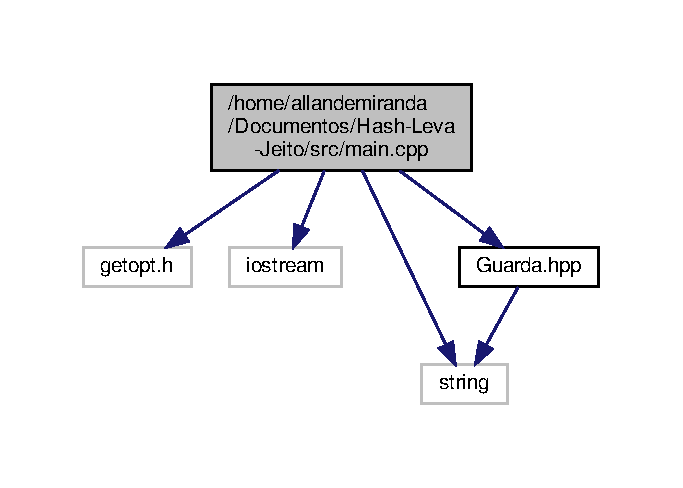
\includegraphics[width=328pt]{da/dce/main_8cpp__incl}
\end{center}
\end{figure}
\subsection*{Functions}
\begin{DoxyCompactItemize}
\item 
int \hyperlink{main_8cpp_a0ddf1224851353fc92bfbff6f499fa97}{main} (int argc, char $\ast$argv\mbox{[}$\,$\mbox{]})
\begin{DoxyCompactList}\small\item\em Função main. \end{DoxyCompactList}\end{DoxyCompactItemize}


\subsection{Detailed Description}
Main. 

\begin{DoxyAuthor}{Author}
Allan de Miranda Silva (\href{mailto:allandemiranda@gmail.com}{\tt allandemiranda@gmail.\+com}) 
\end{DoxyAuthor}
\begin{DoxyVersion}{Version}
0.\+2 
\end{DoxyVersion}
\begin{DoxyDate}{Date}
25-\/09-\/2019
\end{DoxyDate}
\begin{DoxyCopyright}{Copyright}
Copyright (c) 2019 
\end{DoxyCopyright}


\subsection{Function Documentation}
\mbox{\Hypertarget{main_8cpp_a0ddf1224851353fc92bfbff6f499fa97}\label{main_8cpp_a0ddf1224851353fc92bfbff6f499fa97}} 
\index{main.\+cpp@{main.\+cpp}!main@{main}}
\index{main@{main}!main.\+cpp@{main.\+cpp}}
\subsubsection{\texorpdfstring{main()}{main()}}
{\footnotesize\ttfamily int main (\begin{DoxyParamCaption}\item[{int}]{argc,  }\item[{char $\ast$}]{argv\mbox{[}$\,$\mbox{]} }\end{DoxyParamCaption})}



Função main. 


\begin{DoxyParams}{Parameters}
{\em argc} & Quantidade de argumentos \\
\hline
{\em argv} & Argumentos de entrada \\
\hline
\end{DoxyParams}
\begin{DoxyReturn}{Returns}
int return 
\end{DoxyReturn}


Definition at line 24 of file main.\+cpp.


\hypertarget{_open_log_file_8cpp}{}\section{/home/allandemiranda/\+Documentos/\+Hash-\/\+Leva-\/\+Jeito/src/\+Open\+Log\+File.cpp File Reference}
\label{_open_log_file_8cpp}\index{/home/allandemiranda/\+Documentos/\+Hash-\/\+Leva-\/\+Jeito/src/\+Open\+Log\+File.\+cpp@{/home/allandemiranda/\+Documentos/\+Hash-\/\+Leva-\/\+Jeito/src/\+Open\+Log\+File.\+cpp}}


Métodos para a classe \hyperlink{class_open_log_file}{Open\+Log\+File}.  


{\ttfamily \#include \char`\"{}Open\+Log\+File.\+hpp\char`\"{}}\newline
{\ttfamily \#include $<$fstream$>$}\newline
{\ttfamily \#include $<$iostream$>$}\newline
{\ttfamily \#include $<$string$>$}\newline
{\ttfamily \#include $<$vector$>$}\newline
{\ttfamily \#include \char`\"{}Log.\+hpp\char`\"{}}\newline
Include dependency graph for Open\+Log\+File.\+cpp\+:
\nopagebreak
\begin{figure}[H]
\begin{center}
\leavevmode
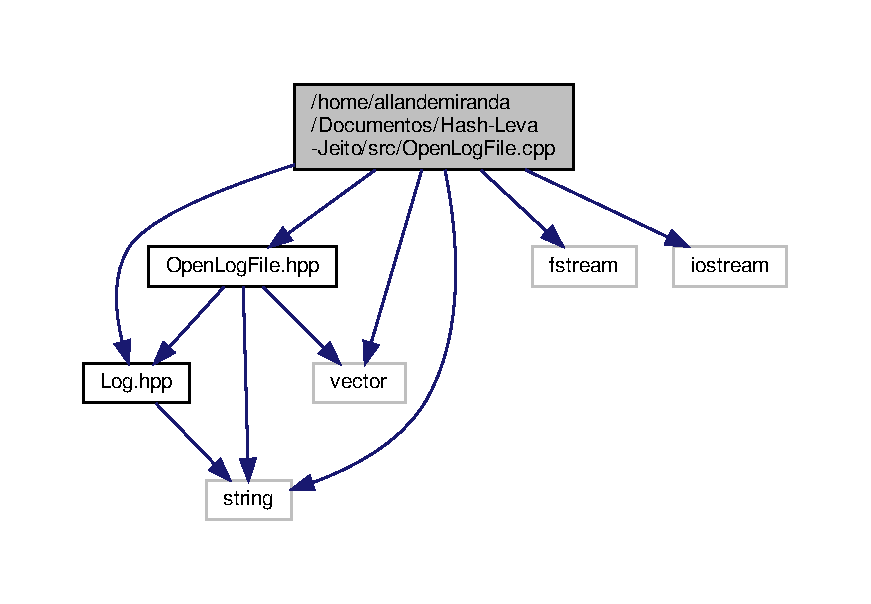
\includegraphics[width=350pt]{d0/d8d/_open_log_file_8cpp__incl}
\end{center}
\end{figure}


\subsection{Detailed Description}
Métodos para a classe \hyperlink{class_open_log_file}{Open\+Log\+File}. 

\begin{DoxyAuthor}{Author}
Allan de Miranda Silva (\href{mailto:allandemiranda@gmail.com}{\tt allandemiranda@gmail.\+com}) 
\end{DoxyAuthor}
\begin{DoxyVersion}{Version}
0.\+1 
\end{DoxyVersion}
\begin{DoxyDate}{Date}
25-\/09-\/2019
\end{DoxyDate}
\begin{DoxyCopyright}{Copyright}
Copyright (c) 2019 
\end{DoxyCopyright}

\hypertarget{_reading_folder_files_8cpp}{}\section{/home/allandemiranda/\+Documentos/\+Hash-\/\+Leva-\/\+Jeito/src/\+Reading\+Folder\+Files.cpp File Reference}
\label{_reading_folder_files_8cpp}\index{/home/allandemiranda/\+Documentos/\+Hash-\/\+Leva-\/\+Jeito/src/\+Reading\+Folder\+Files.\+cpp@{/home/allandemiranda/\+Documentos/\+Hash-\/\+Leva-\/\+Jeito/src/\+Reading\+Folder\+Files.\+cpp}}


Métodos da classe \hyperlink{class_reading_folder_files}{Reading\+Folder\+Files}.  


{\ttfamily \#include \char`\"{}Reading\+Folder\+Files.\+hpp\char`\"{}}\newline
{\ttfamily \#include $<$dirent.\+h$>$}\newline
{\ttfamily \#include $<$cstdlib$>$}\newline
{\ttfamily \#include $<$string$>$}\newline
{\ttfamily \#include $<$vector$>$}\newline
Include dependency graph for Reading\+Folder\+Files.\+cpp\+:
\nopagebreak
\begin{figure}[H]
\begin{center}
\leavevmode
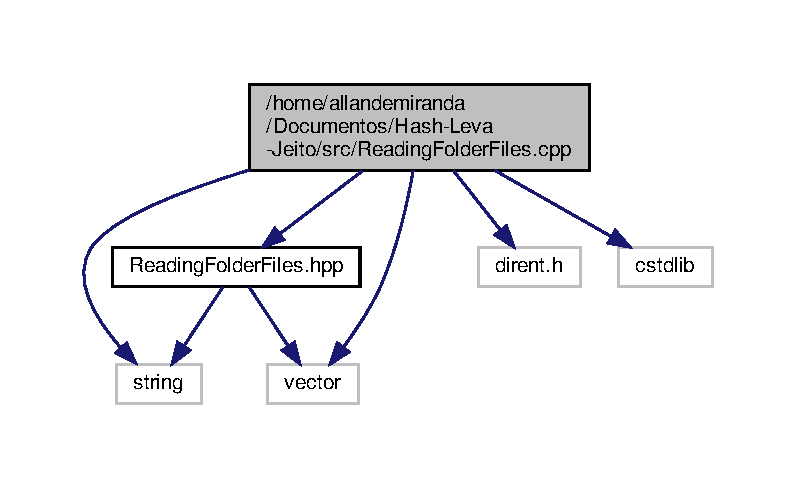
\includegraphics[width=350pt]{d6/d48/_reading_folder_files_8cpp__incl}
\end{center}
\end{figure}


\subsection{Detailed Description}
Métodos da classe \hyperlink{class_reading_folder_files}{Reading\+Folder\+Files}. 

\begin{DoxyAuthor}{Author}
Allan de Miranda Silva (\href{mailto:allandemiranda@gmail.com}{\tt allandemiranda@gmail.\+com}) 
\end{DoxyAuthor}
\begin{DoxyVersion}{Version}
0.\+1 
\end{DoxyVersion}
\begin{DoxyDate}{Date}
25-\/09-\/2019
\end{DoxyDate}
\begin{DoxyCopyright}{Copyright}
Copyright (c) 2019 
\end{DoxyCopyright}

\hypertarget{_report_output_8cpp}{}\section{/home/allandemiranda/\+Documentos/\+Hash-\/\+Leva-\/\+Jeito/src/\+Report\+Output.cpp File Reference}
\label{_report_output_8cpp}\index{/home/allandemiranda/\+Documentos/\+Hash-\/\+Leva-\/\+Jeito/src/\+Report\+Output.\+cpp@{/home/allandemiranda/\+Documentos/\+Hash-\/\+Leva-\/\+Jeito/src/\+Report\+Output.\+cpp}}


Métodos para a classe \hyperlink{class_report_output}{Report\+Output}.  


{\ttfamily \#include \char`\"{}Report\+Output.\+hpp\char`\"{}}\newline
{\ttfamily \#include $<$dirent.\+h$>$}\newline
{\ttfamily \#include $<$cstring$>$}\newline
{\ttfamily \#include $<$fstream$>$}\newline
{\ttfamily \#include $<$iostream$>$}\newline
{\ttfamily \#include $<$string$>$}\newline
{\ttfamily \#include $<$vector$>$}\newline
{\ttfamily \#include \char`\"{}Log.\+hpp\char`\"{}}\newline
Include dependency graph for Report\+Output.\+cpp\+:
\nopagebreak
\begin{figure}[H]
\begin{center}
\leavevmode
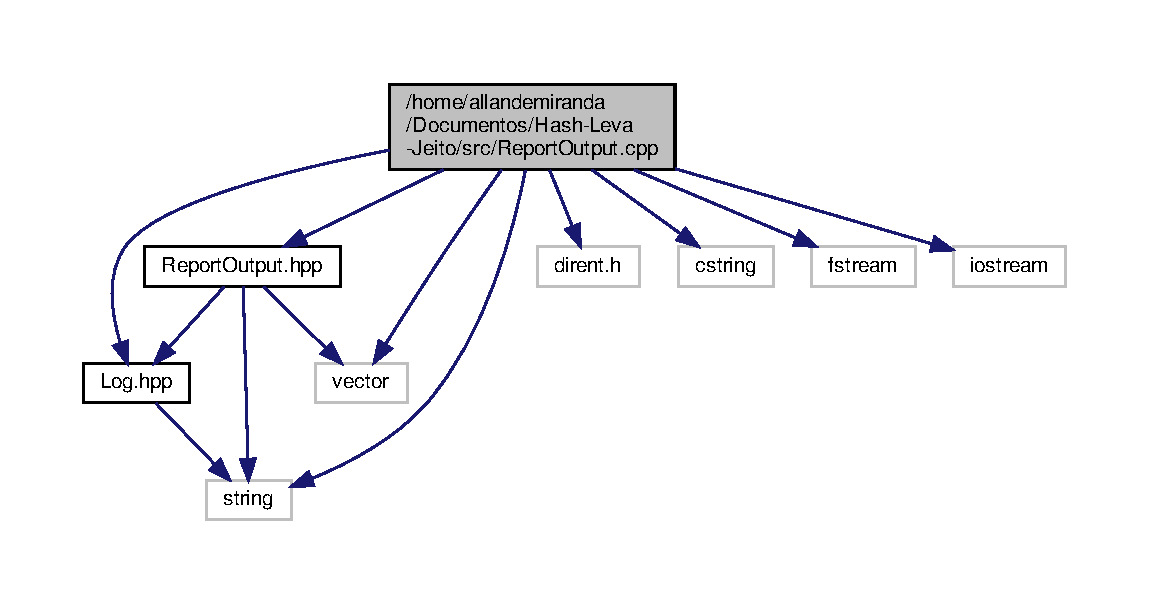
\includegraphics[width=350pt]{d6/d26/_report_output_8cpp__incl}
\end{center}
\end{figure}


\subsection{Detailed Description}
Métodos para a classe \hyperlink{class_report_output}{Report\+Output}. 

\begin{DoxyAuthor}{Author}
Allan de Miranda Silva (\href{mailto:allandemiranda@gmail.com}{\tt allandemiranda@gmail.\+com}) 
\end{DoxyAuthor}
\begin{DoxyVersion}{Version}
0.\+1 
\end{DoxyVersion}
\begin{DoxyDate}{Date}
25-\/09-\/2019
\end{DoxyDate}
\begin{DoxyCopyright}{Copyright}
Copyright (c) 2019 
\end{DoxyCopyright}

%--- End generated contents ---

% Index
\backmatter
\newpage
\phantomsection
\clearemptydoublepage
\addcontentsline{toc}{chapter}{Index}
\printindex

\end{document}
